%%%%%%%%%%%%%%%%%%%%%%%%%%%%%%%%%%%%%%%%%%%%%%%%%%%%%%%%%%%%%%%%%%%%
%%%%%%%%%%%%%%%%%%%%%%%%%%%%%%%%%%%%%%%%%%%%%%%%%%%%%%%%%%%%%%%%%%%%
%%                                                                %%
%% An example for writting your thesis using LaTeX                %%
%% Original version by Luis Costa,  changes by Perttu Puska       %%
%% Support for Swedish added 15092014                             %%
%%                                                                %%
%% This example consists of the files                             %%
%%         thesistemplate.tex (versio 2.01)                       %%
%%         opinnaytepohja.tex (versio 2.01) (for text in Finnish) %%
%%         aaltothesis.cls (versio 2.01)                          %%
%%         kuva1.eps                                              %%
%%         kuva2.eps                                              %%
%%         kuva1.pdf                                              %%
%%         kuva2.pdf                                              %%
%%                                                                %%
%%                                                                %%
%% Typeset either with                                            %%
%% latex:                                                         %%
%%             $ latex opinnaytepohja                             %%
%%             $ latex opinnaytepohja                             %%
%%                                                                %%
%%   Result is the file opinnayte.dvi, which                      %%
%%   is converted to ps format as follows:                        %%
%%                                                                %%
%%             $ dvips opinnaytepohja -o                          %%
%%                                                                %%
%%   and then to pdf as follows:                                  %%
%%                                                                %%
%%             $ ps2pdf opinnaytepohja.ps                         %%
%%                                                                %%
%% Or                                                             %%
%% pdflatex:                                                      %%
%%             $ pdflatex opinnaytepohja                          %%
%%             $ pdflatex opinnaytepohja                          %%
%%                                                                %%
%%   Result is the file opinnaytepohja.pdf                        %%
%%                                                                %%
%% Explanatory comments in this example begin with                %%
%% the characters %%, and changes that the user can make          %%
%% with the character %                                           %%
%%                                                                %%
%%%%%%%%%%%%%%%%%%%%%%%%%%%%%%%%%%%%%%%%%%%%%%%%%%%%%%%%%%%%%%%%%%%%
%%%%%%%%%%%%%%%%%%%%%%%%%%%%%%%%%%%%%%%%%%%%%%%%%%%%%%%%%%%%%%%%%%%%

%% Uncomment one of these:
%% the 1st when using pdflatex, which directly typesets your document in
%% pdf (use jpg or pdf figures), or
%% the 2nd when producing a ps file (use eps figures, don't use ps figures!).
\documentclass[english,12pt,a4paper,pdftex,elec,utf8]{aaltothesis}
%\documentclass[english,12pt,a4paper,dvips]{aaltothesis}

%% To the \documentclass above
%% specify your school: arts, biz, chem, elec, eng, sci
%% specify the character encoding scheme used by your editor: utf8, latin1

%% Use one of these if you write in Finnish (see the Finnish template):
%%
%\documentclass[finnish,12pt,a4paper,pdftex,elec,utf8]{aaltothesis}
%\documentclass[finnish,12pt,a4paper,dvips]{aaltothesis}

\usepackage{graphicx}

%% Use this if you write hard core mathematics, these are usually needed
\usepackage{amsfonts,amssymb,amsbsy}

%includes amsmath for EQREF
\usepackage{mathtools}


%% Use the macros in this package to change how the hyperref package below 
%% typesets its hypertext -- hyperlink colour, font, etc. See the package
%% documentation. It also defines the \url macro, so use the package when 
%% not using the hyperref package.
%%
%\usepackage{url}

%% Use this if you want to get links and nice output. Works well with pdflatex.
\usepackage{hyperref}
\hypersetup{pdfpagemode=UseNone, pdfstartview=FitH,
  colorlinks=true,urlcolor=red,linkcolor=blue,citecolor=black,
  pdftitle={Energy Harvester Design for Intelligent Tyre Systems},pdfauthor={Otso Jousimaa},
  pdfkeywords={Modify keywords}}

%Use for degree symbol
\usepackage{gensymb}

%for color
\usepackage{color}

%for block comments
\usepackage{verbatim}


%% All that is printed on paper starts here
\begin{document}

%% Change the school field to specify your school if the automatically 
%% set name is wrong
% \university{aalto-yliopisto}
\university{Aalto University}
% \school{Sähkötekniikan korkeakoulu}
\school{School of Electrical Engineering}

%% Only for B.Sc. thesis: Choose your degree programme. 
%\degreeprogram{Electronics and electrical engineering}
%%

%% ONLY FOR M.Sc. AND LICENTIATE THESIS: Specify your department,
%% professorship and professorship code. 
%%
\department{Department of Automation and Systems Technology}
\professorship{Smart products}
%%

%% Valitse yksi näistä kolmesta
%%
%% Choose one of these:
%\univdegree{BSc}
\univdegree{MSc}
%\univdegree{Lic}

%% Your own name (should be self explanatory...)
\author{Otso Jousimaa}

%% Your thesis title comes here and again before a possible abstract in
%% Finnish or Swedish . If the title is very long and latex does an
%% unsatisfactory job of breaking the lines, you will have to force a
%% linebreak with the \\ control character. 
%% Do not hyphenate titles.
%% 
\thesistitle{Energy Harvester Design for Intelligent Tyre Systems}

\place{Espoo}

%% For B.Sc. thesis use the date when you present your thesis. 
%% 
%% Kandidaatintyön päivämäärä on sen esityspäivämäärä! 
\date{XX.XX.XXXX}

%% B.Sc. or M.Sc. thesis supervisor 
%% Note the "\" after the comma. This forces the following space to be 
%% a normal interword space, not the space that starts a new sentence. 
%% This is done because the fullstop isn't the end of the sentence that
%% should be followed by a slightly longer space but is to be followed
%% by a regular space.
%%
\supervisor{Prof.\ Arto Visala} %{Prof.\ Pirjo Professori}

%% B.Sc. or M.Sc. thesis advisors(s). You can give upto two advisors in
%% this template. Check with your supervisor how many official advisors
%% you can have.
%%
%\advisor{Prof.\ Pirjo Professori}
\advisor{M.Sc.\ Yi Xiong}
\advisor{D.Sc.\ (Tech.) Ari Tuononen}

%% Aalto logo: syntax:
%% \uselogo{aaltoRed|aaltoBlue|aaltoYellow|aaltoGray|aaltoGrayScale}{?|!|''}
%%
%% Logo language is set to be the same as the document language.
%% Logon kieli on sama kuin dokumentin kieli
%%
\uselogo{aaltoRed}{''}

%% Create the coverpage
%%
\makecoverpage


%% Note that when writting your master's thesis in English, place
%% the English abstract first followed by the possible Finnish abstract

%% English abstract.
%% All the information required in the abstract (your name, thesis title, etc.)
%% is used as specified above.
%% Specify keywords
%%
%% Kaikki tiivistelmässä tarvittava tieto (nimesi, työnnimi, jne.) käytetään
%% niin kuin se on yllä määritelty.
%% Avainsanat
%%
\keywords{For keywords choose concepts that are central to your thesis}
%% Abstract text
\begin{abstractpage}[english]
  Your abstract in English. Try to keep the abstract short; approximately 
  100 words should be enough. The abstract explains your research topic, 
  the methods you have used, and the results you obtained.  
  Your abstract in English. Try to keep the abstract short; approximately 
  100 words should be enough. The abstract explains your research topic, 
  the methods you have used, and the results you obtained.  

  Your abstract in English. Try to keep the abstract short; approximately 
  100 words should be enough. The abstract explains your research topic, 
  the methods you have used, and the results you obtained.  
  Your abstract in English. Try to keep the abstract short; approximately 
  100 words should be enough. The abstract explains your research topic, 
  the methods you have used, and the results you obtained.  
\end{abstractpage}

%% Force a new page so that the possible English abstract starts on a new page
%%
%% Pakotetaan uusi sivu varmuuden vuoksi, jotta 
%% mahdollinen suomenkielinen ja englanninkielinen tiivistelmä
%% eivät tule vahingossakaan samalle sivulle
\newpage
%
%% Abstract in Finnish.  Delete if you don't need it. 
\thesistitle{Energy Harvester Design for Intelligent Tire Systems}
\advisor{DI Yi Xiong}
\advisor{TkT Ari Tuononen}
\degreeprogram{Automaatio- ja systeemitekniikka}
\department{Automaatio- ja systeemitekniikan laitos}
\professorship{Älykkäät tuotteet}
%% Avainsanat
\keywords{Vastus, Resistanssi,\\ Lämpötila}
%% Tiivistelmän tekstiosa
\begin{abstractpage}[finnish]
  Tiivistelmässä on lyhyt selvitys (noin 100 sanaa)
  kirjoituksen tärkeimmästä sisällöstä: mitä ja miten on tutkittu,
  sekä mitä tuloksia on saatu. 
  Tiivistelmässä on lyhyt selvitys (noin 100 sanaa)
  kirjoituksen tärkeimmästä sisällöstä: mitä ja miten on tutkittu,
  sekä mitä tuloksia on saatu. 

  Tiivistelmässä on lyhyt selvitys (noin 100 sanaa)
  kirjoituksen tärkeimmästä sisällöstä: mitä ja miten on tutkittu,
  sekä mitä tuloksia on saatu. 
  Tiivistelmässä on lyhyt selvitys (noin 100 sanaa)
  kirjoituksen tärkeimmästä sisällöstä: mitä ja miten on tutkittu,
  sekä mitä tuloksia on saatu. 
  Tiivistelmässä on lyhyt selvitys (noin 100 sanaa)
  kirjoituksen tärkeimmästä sisällöstä: mitä ja miten on tutkittu,
  sekä mitä tuloksia on saatu. 
\end{abstractpage}


%% Preface
%%
%% Esipuhe 
\mysection{Preface}
%\mysection{Esipuhe}
I want to thank Professor Pirjo Professori
and my instructor Olli Ohjaaja for their 
good and poor guidance.\\

\vspace{5cm}
Otaniemi, 16.1.2015

\vspace{5mm}
{\hfill Eddie E.\ A.\ Engineer \hspace{1cm}}

%% Force new page after preface
%%
%% Pakotetaan varmuuden vuoksi esipuheen jälkeinen osa
%% alkamaan uudelta sivulta
\newpage


%% Table of contents. 
\thesistableofcontents


%% Symbols and abbreviations
\mysection{Symbols and abbreviations}

\subsection*{Symbols}

\begin{tabular}{ll}
$\mathbf{A}$  & area \\
$\mathbf{B}$  & magnetic flux density  \\
$c$           & speed of light in vacuum $\approx 3\times10^8$ [m/s]\\
$\varepsilon$ & electromotive force \\
$\mathbf{F}$  & mechanical force \\
$\mathbf{I}$  & electrical current \\
$\mathbf{l}$  & length \\
$\Phi_{B}$    & magnetic flux through loop area \\
$\rho$        & resistivity \\
$\mathbf{P}$  & power \\
$\mathbf{p}$  & pressure \\
$\mathbf{U}$  & input to system \\
$\mathbf{V}$  & voltage \\
$\mathbf{Y}$  & output from system \\
$\mathbf{Z}$  & complex impedance
\end{tabular}

\subsection*{Operators}

\begin{tabular}{ll}
$\displaystyle\frac{\mbox{d}}{\mbox{d} t}$ & derivative with respect to 
variable $t$\\[3mm]
$\displaystyle\frac{\partial}{\partial t}$  & partial derivative with respect 
to variable $t$ \\[3mm]
$\sum_i $                       & sum over index $i$
\end{tabular}

\subsection*{Abbreviations}

\begin{tabular}{ll}
AC         & Alternating Current \\
BLE        & Bluetooth Low Energy \\
DC         & Direct Current \\
EMF        & Electromotive Force \\
IC         & Integrated Circuit \\
MEMS       & Microelectromechanical Systems \\
MPPT       & Maximum Power Point Tracking \\
PV         & Photovoltaic \\
RF         & Radio Frequency \\
SMPS       & Switch-Mode Power Supply \\
TPMS       & Tire Pressure Monitoring Sensors
\end{tabular}


%% Tweaks the page numbering to meet the requirement of the thesis format:
%% Begin the pagenumbering in Arabian numerals (and leave the first page
%% of the text body empty, see \thispagestyle{empty} below).
%% Additionally, force the actual text to begin on a new page with the 
%% \clearpage command.
%% \clearpage is similar to \newpage, but it also flushes the floats (figures
%% and tables).
%% There is no need to change these
%%
\cleardoublepage
\storeinipagenumber
\pagenumbering{arabic}
\setcounter{page}{1}


%% Text body begins. Note that since the text body
%% is mostly in Finnish the majority of comments are
%% also in Finnish after this point. There is no point in explaining
%% Finnish-language specific thesis conventions in English. Someday 
%% this text will possibly be translated to English.
%%
%\section{Introduction}
\section{Introduction}

%% 
%% Leave first page empty
\thispagestyle{empty}

As technology advances, it becomes possible to build small, light-weight and yet powerful sensor platforms which can communicate wirelessly within their environment. New kind of applications are being created using the possibilities given by these sensor platforms. A common trait with all of these devices is that they need power to function, even if the power needed is minuscule. 

Traditionally wireless devices have been powered by batteries, but as the number of sensors increases, the cost of changing or charging the batteries becomes a significant part of the cost of such system. This is especially relevant for the devices which are in hard to reach areas, such as internal parts of heavy machinery, walls of bridges, high rise buildings, remote environmental sensors et cetera. In some cases the life of the battery can become a limiting factor for the lifetime of entire sensor, if the cost of installing new sensor is similar to cost of replacing the battery.

A new approach to powering devices is to harvest the energy from their surroundings using ambient energy as the power source. Examples of energy sources are solar, wind, temperature differentials and vibration. The technology to utilise wind and solar is already widely deployed and even used in large-scale power production. On a smaller scale the demand for reliable and efficient solutions has been growing steadily with the advent of low-power wireless devices. A lot of research has focused on creating suitable technologies and devices for low-power energy harvesting. 

This work focuses on powering one of such devices, namely a sensor inside a car tyre. The car tyre provides some unique challenges and opportunities, as there is a lot of energy available, but on the other hand operating conditions can be extremely harsh with large temperature ranges, extreme vibration and shocks especially in rougher road conditions.

Car tyre sensing itself has been in focus of a lot development lately, as legislation in the United States demand new cars being fitted with a pressure sensor to warn drivers about low pressure causing higher fuel consumption, wear on tyre and even elevated risk of accidents. The European Union also has laws which require Tyre Pressure Monitoring Sensors (TPMS) on new passenger cars. 

This thesis provides a cursory view into current energy harvesting technologies and operational environment. Next section presents background of the field, Section \ref{sect:design} presents a design process for an electromagnetic and a piezoelectric energy harvesting system for car tyres. The results of the systems are presented in Section \ref{sect:results}, where both methods were found to produce meaningful power levels. Conclusions of the work can be found in Section \ref{sect:conclusions}. All the original material created for this Thesis can be found at https://github.com/ojousima/thesis. 


%\section{Background}
%% In a thesis, every section starts a new page, hence \clearpage
\clearpage
\section{Background}

\subsection{Structure of a tyre}

\subsection{Environment inside tyre}
The energy harvester will be placed inside the tyre. Previous studies by Niskanen et al \cite{Niskanen2014}. have shown that the tyre will experience acceleration in all three axes. Tangential and centripetal accelerations are dominant, they can reach amplitudes of up to 150 g in test fixture. In addition a study done by Löhndorf et al. \cite{Lohndorf2007} shows shock survival of up to 4 000 - 5 000 g is required for reliability. 

Temperature inside of the tire will reach equilliberium in ambient + 5-10 \degree C, so operation temperature should be in range of -40 to + 75 \degree C to have some safety margin on top of usual Finnish ambient conditions {\color{red} reasonable tempetature range?}.

Previous work \cite{Niskanen2014} was used to as a basis for analysis of characteristics of acceleration inside tire. Raw data was used to gather minimum and maximum values of acceleration as well as frequency components inside tire. Data was gathered at 20 km/h, 60 km/h and 80 km/h speeds. 

Figures \ref{80_TD} and \ref{80_TD_zoom} are time domain representations of the acceleration along 3 axes as shown in figure \ref{tyre_axes}. First figure shows 10 rotations of tyre, contact with drum is clearly visible as a sudden shock. Second figure is a zoom into one rotation.

\begin{figure}[htb]
\begin{center}
\includegraphics[height=4cm]{images/cited/matilainen2012}
\end{center}
\caption{Axes in measurement by Matilainen et al. \cite{Matilainen2012}}
\label{80_TD}
\end{figure}

Frequency domain representations were calculated in Matlab. There are two main contributors to base frequencies: first is the rotational frequency of tyre itself and second is the impact when the tyre deforms as it contacts the drum.. There is clearly visible series of frequency components spaced at the rotational frequency of tyre as well as shock harmonics at upper frequencies. Figures \ref{80_FFT} and \ref{80_FFT_zoom} show the total frequency spectrum and the dominant frequency components. {\color{red} Images to be redrawn, labeled properly, font size increased, combined into one. Check the windowing.}.

\begin{figure}[htb]
\begin{center}
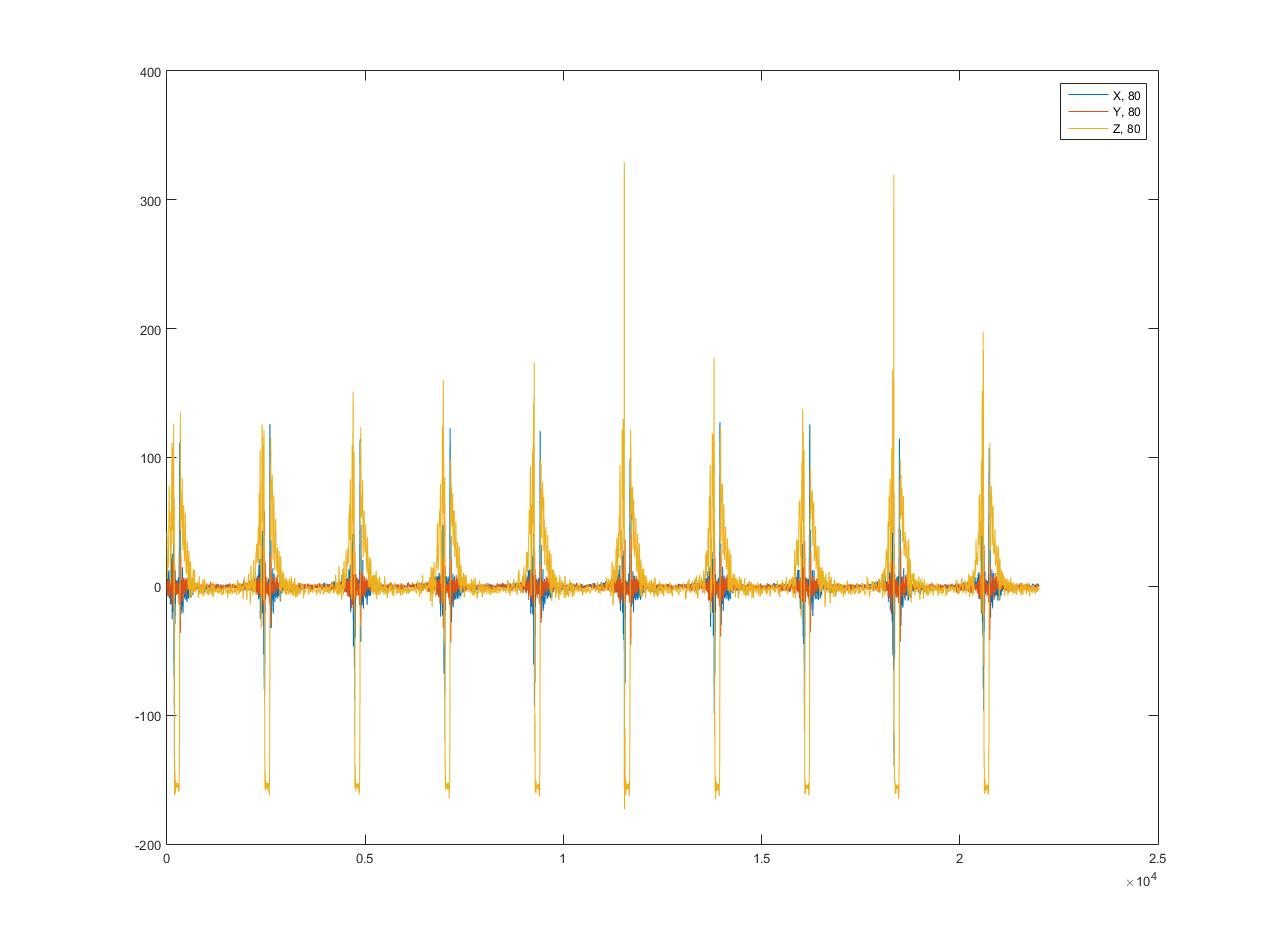
\includegraphics[height=4cm]{images/80kmh_timedomain}
\end{center}
\caption{Acceleration of inner lining of tyre at 80 km/h in time domain.}
\label{80_TD}
\end{figure}

\begin{figure}[htb]
\begin{center}
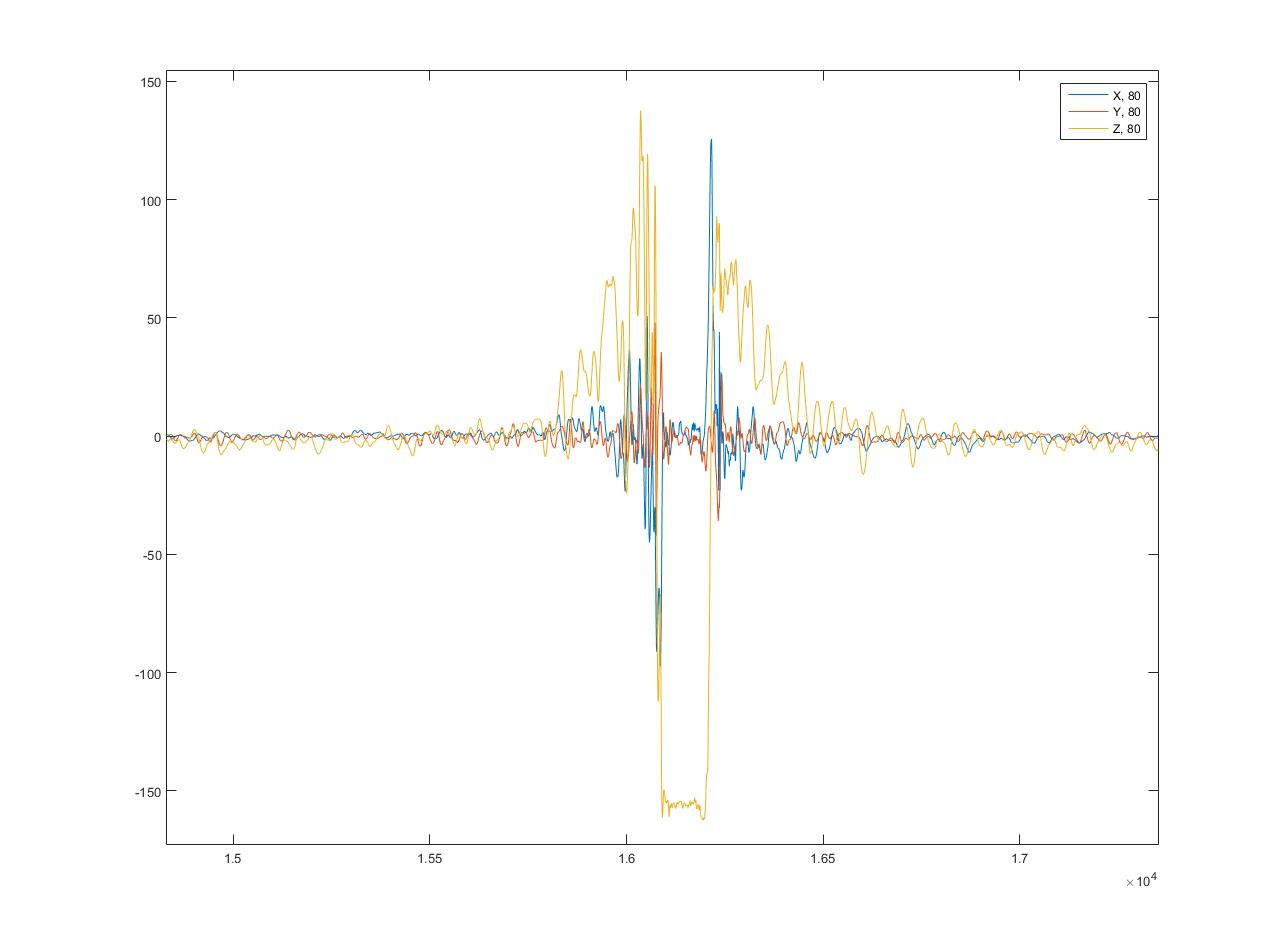
\includegraphics[height=4cm]{images/80kmh_timedomain_onerotation}
\end{center}
\caption{Acceleration of tyre inner lining in single rotation at 80 km/h. }
\label{80_TD_zoom}
\end{figure}

\begin{figure}[htb]
\begin{center}
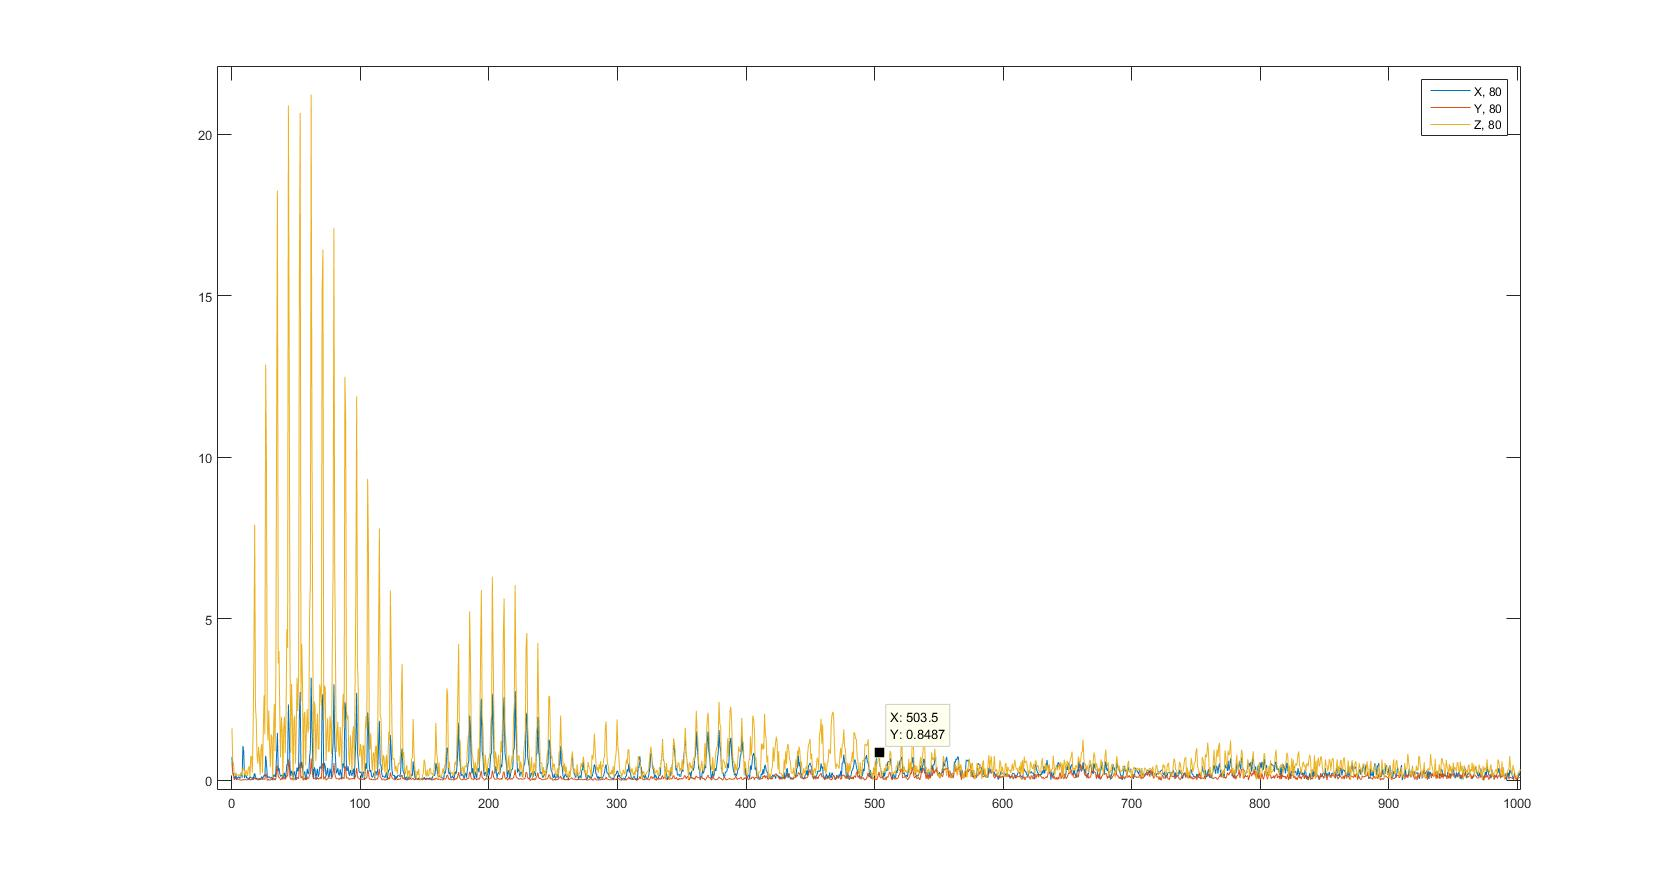
\includegraphics[height=4cm]{images/FFT-80}
\end{center}
\caption{Frequency domain representation of acceleration data.}
\label{80_FFT}
\end{figure}

\begin{figure}[htb]
\begin{center}
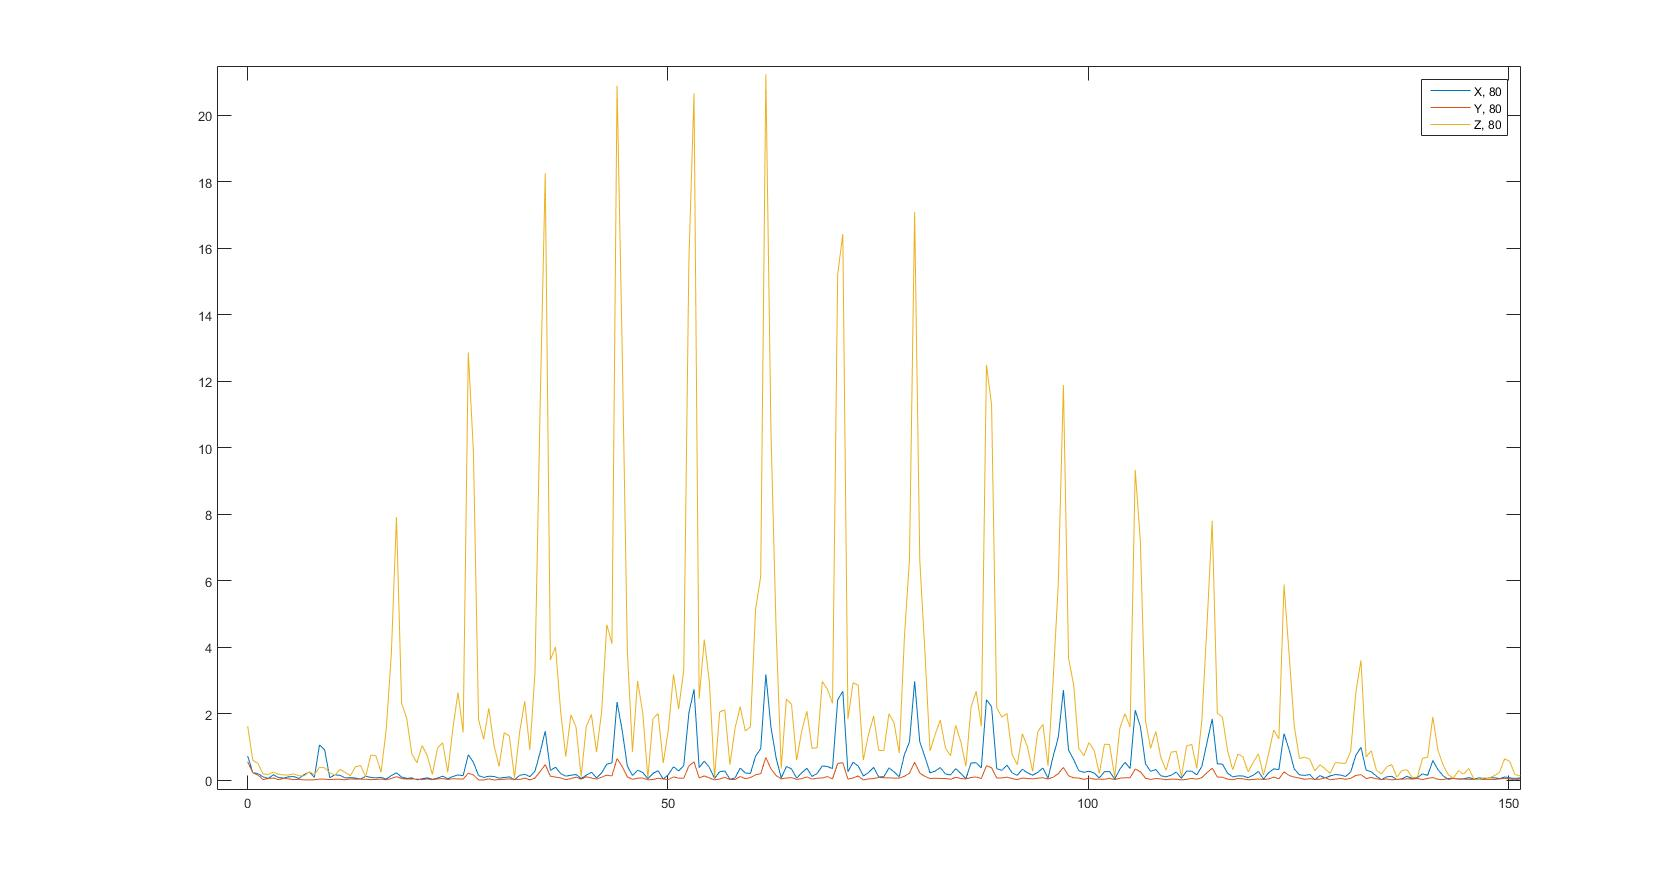
\includegraphics[height=4cm]{images/FFT-80-zoom}
\end{center}
\caption{Most of the energy is found in 10-100 Hz range.}
\label{80_FFT_zoom}
\end{figure}

It's important to notice that the sensor used was piezoelectric, which forms a highpass filter as the operation is based on charge between layers. This charge dissipates over time, so the steady-state centripetal acceleration reads as zero. There is a constant acceleration on the device caused by rotational movement by the tire. 

\subsection{Energy harvesting}
\subsubsection{Overview of methods}
First step of designing a system for energy harvesting was to identify the currently known methods and their properties. Kubba et al. \cite{Kubba2014} have done a study on tyre pressure sensor technology, they present electromagnetic, electrostatic, piezoelectric and thermal solutions as possible candidates for energy harvesting. In addition, triboelectric and magnetostrictive methods have been proposed by Bowen et al \cite{Bowen2014}. Outside of the context of tyres, Paradiso et al. \cite{Paradiso2005} present solar and radiowave harvesting techniques. Radioactive power source has been suggested by Lal et al \cite{Lal2004}. 

Electromagnetic power sources are based on Faraday's law of electromagnetic induction. A magnet and a coil are put in motion relative to each other, and the changing magnetic flux through the coils of the generator produces voltage. Current through such device is determined by load resistance. Technology is widely used in power generation, where a primary power source such as wind or flow of water provides rotation for the generator. While conventional designs use rotational movement, linear generator designs exist. Boldea and Nasar \cite{Boldea1999} provide an overview of linear generator and actuator theory. 

Electrostatic devices charge plates of a capacitor and use mechanical vibration to vary the structure of the capacitor. As the capacitance value changes with the structure, energy can be harvested from increased potential energy in capacitor. Drawback of this method is the required control electronics and high polarization voltages needed for maximal efficiency. There are also electrostatic methods which use electrets. These electrects hold constant charge and polarization for years and they can be used in electrostatic harvesters which do not require an external exitation source \cite{Boisseau2012}. As electret elements and electrostatic generators are not readily available, they have been excluded from this study.

Piezoelectric materials generate charge in response of mechanical stress. This stress can be caused by firmly attaching the piezoelectric element to a surface which deforms (simply supported) or by leaving one end of the element free-hanging while other end is fixed (cantilevered). Dynamics of the generator are very different for the different configurations, Kim et al. \cite{Kim2014a} provides a model for impact-based piezoelectric harvester while Erturk et al. have done in-depth analysis of cantilevered piezoelectric modeling \cite{Erturk2009}. 

Thermal solutions can be further diveded into subcategories. Seeback-effect where a temperature gradient in a semiconductor material causes voltage between poles of the material is widely used in temperature sensing, but to generate appreciable amounts of power large temperature gradients of over hundred \degree C are required \cite{Amatya2010} which is not practical inside tyre. Pyroelectric materials do not require differential of temperature, they generate energy when the temperature of the entire element changes \cite{Zhang2011}. As the temperature inside tyre remains rather constant over long periods of time, these methods are not practical for this application.

Triboelectricity generates power using friction between two materials, a classic example of this is Benjamin Franklin's experiments on charging various rods by rubbing them against different materials. A flexible triboelectric generator has been presented by Fan et al. \cite{Fan2012}. Triboelectric sheets are not readily available and their construction is complex, so triboelectric generation is excluded from this work. 

Magnetostrictive materials change their magnetic field in response to external mechanical sterss. This change can be utilised to create a magnetic flux through coils as in electromagnetic generators. A magnetostrictive generator was built by Wang et al. \cite{Wang2006}. 

Solar energy can be harvested by using sun as a energy source for a thermal energy harvesting or by utilizing the photovoltaic effect to generate electricity from photons hitting photovoltaic material. Photovoltaic technology is mature and widely used, but as there is no source of light inside tyre, photovoltaic methods are not suited for the application.

Radio wave harvesting uses antennas to collect energy from ambient radio transmissions, such as WiFi- and cellural signals. Patel et al \cite{Patel2014} have built a demonstration device which uses TV broadcasts as an energy source. The tyre material dampens any RF broadcasts, which makes RF energy harvesting poorly suited for the application.

Radioactive energy harvesting resembles battery or fuel cell. A radioactive material is deposited in generator near piezoelectric cantilever. Radioactive decay charges proof mass of piezoelectric cantilever until the proof mass contacts the radioactive material by electrostatic attaraction, at which point the electrical charge is balanced and piezoelectric beam begins resonant vibration as in normal piezoelectric harvesting. Such a battery has lifetime limited only by half-life of the used material. Lal and Blanchard \cite{Lal2004} present such a battery. This kind of battery would be redundant for the application, as there already exists energy in rotation of tyre which can be used to energise the cantilever. 

In conclusion, a wide range of energy harvesting technologies have been identified. As their primary properties are known, we can narrow down the suitable technology to electromagnetic, piezoelectric and magnetostrictive. These technologies are studied further to identify optimal choice for the application.

\subsubsection{Resonance-based piezoelectric harvesting}
Piezoelectric materials produce voltage in response to mechanical stress. The effect is bidirectional, piezoelectric element can also produce mechanical strain in response to applied voltage. The material has crystalline structure with electrical dipoles in balanced state when no stress is applied. Mechanical stress unbalances these dipoles, creating element which resembles electronically a charged capacitor. 

A common approach to piezoelectric harvesting is to configure the element as a cantilever and tune the resonant frequency of the system to dominant frequency of the surrounding environment. In some applications, such as in machines running at the frequency of power grid (50 HZ or 60 HZ) this kind of frequency-tuning is relatively straightforward. TODO

\subsubsection{Impact-based piezoelectric harvesting}
As the resonant harvesting is not feasible in the environment inside tire, another method would be to use an impactor to hit a piezoelectric plate on every cycle of a tire. These impacts would provide energy once per rotation of a tire. This method has been tried before by {\color{red} Cite} and it was found to provide up to 4 mW of power in average. TODO

\subsubsection{Electromagnetical harvesting}
Electromagnetical harvesting is based on Faraday's law of induction: A loop of wire acquires electromotive force (EMF) in response to a changing magnetic field. More formally:

\begin{equation}
  \varepsilon = - \frac{d \Phi_ {B}}{d t} , 
\end{equation}

where $\varepsilon$ is the EMF, $\Phi_{B}$ is magnetic flux through loop area, and $t$ is time. For a tightly wound coil of wire, the equation can be stated as 

\begin{equation} \label{eq:emf}
  \varepsilon = -N \frac{d \Phi_{B}}{d t} , 
\end{equation}

where N is the number of turns in a coil. \cite[p.999]{universityphysics}

It's important to notice that magnetic flux through wire $ \Phi_{B} $ can change for a variety of reasons: the source of field can be in motion, strength of field can vary, the coil can be in motion, and the shape of coil can vary. In energy harvesting application in an environment with vibrations motional energy is readily available, so we focus on energy harvesting methods which either move the source of magnetic field or the coil itself.

It's obvious from equation \eqref{eq:emf} that energy available increases with the strength of magnetic source, number of turns in a coil and rate of change in the magnetic field. 

Magnetic source can be either permanent magnet or a electrically induced source as in induction motors. Induction-based generators require reactive power to start up, which means that any harvester design incorporating an induction generator would need a secondary power source to start the inductive generator. Hence the focus of this thesis will be in permanent magnet designs.

In addition to voltage available from the generator, it's important to consider source impedance. A very simple electrical equivalent model of the generator is presented in \ref{gen_simple}, where generator is presented as a voltage source in series with lumped inductor and resistor \cite{Jirutitijaroen2012}. 

\begin{figure}[htb]
\begin{center}
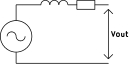
\includegraphics[height=2cm]{images/own_dwg/gen_simple}
\end{center}
\caption{A simple electromachanical generator equivalent circuit.}.
\label{gen_simple}
\end{figure}

This model is greatly simplified and it does not account for factors such as effect of electromagnetical force on mechanical structure of the generator. Even with these limitations, model is still useful as it can be used to determine an optimal load for the generator. 

The power output can be written formally as:

\begin{equation} \label{eq:gen_simple_power}
  P_{generated}(s) = \varepsilon(s)*I_{generated}(s),
\end{equation}

where $P_{generated}(s), V_{generated}(s), I_{generated}(s)$ are complex laplace-domain power, voltage and current dependent on frequency. It can be seen that power is generated only when there is a load available, as without load there is no current flow into our out of generator. Voltage is determined by EMF as described above. Current can be written as: 

\begin{equation} \label{eq:gen_simple_current}
  I_{generated}(s) = \frac{\varepsilon(s)}{Z_{generator}(s)+Z_{load}(s)},
\end{equation}

where substituting $Z_{generator}(s) $ and $ Z_{load}(s)$ are complex impedances of load and generator. This equation is valid only for linear systems, so for example rectifying and converting power with switch mode power supply (SMPS) reduces accuracy of the equation. Substituting \eqref{eq:gen_simple_current} into \eqref{eq:gen_simple_power} we obtain:

\begin{equation}
  P_{generated}(s) = \varepsilon(s)*\frac{\varepsilon(s)}{Z_{generator}(s)+Z_{load}(s)}.
\end{equation}

Total power into load can be written as:

\begin{equation} \label{eq:generator_load_power}
  P_{load}(s) = V_{generated}(s)*\frac{Z_{load}(s)}{Z_{generator}(s)+Z_{load}(s)}*\frac{V_{generated}(s)}{Z_{generator}(s)+Z_{load}(s)}.
\end{equation}

It's easy to see from \eqref{eq:generator_load_power} that if load impedance is infinite or zero, there is no power generated. It can be shown that maximum power is generated when $Z_{generator}(s) = {Z_{load}(s)}^*$. Another consideration is efficiency of the generator. The electrical efficiency is defined as ratio of power flowing into load and total power generated. It's easily seen from equation \eqref{eq:generator_load_power} that when load impedance is equal to generator impedance, efficiency is $ 50 \%$. Efficiency rises with the load impedance, which is why generators are rarely run at their maximum power. In our application the harvested power is minuscule compared to power available in tire, so it makes sense to try to match the load impedance for maximum power.

In energy harvesting application it is important to consider the validity of established theory when generator is scaled to centimetres or even smaller dimensions. Many assumptions, such as coil being tightly wound and made of thin wire might become invalid at microscale. O'Donnel et al. \cite{ODonnell2007} have done a study on the effects of scaling dimensions downwards down to millimetre range, and they concluded that power available from generator is proportional to fourth power of generator dimension for cubical generators. Another of their primary findings was that a microfabricated generator becomes more effective than a traditional wire-wound generator when design is scaled below $2 mm$ length or in $8 mm^3$ volume. It can be concluded that in this application it is reasonable to use a wire-wound generator over microfabricated one, as the generator dimensions can be an order of magnitude larger than this crossover point. 

\subsubsection{Magnetostrictive harvesting}
TODO: Magnetostrictive harvesting resembles piezoelectric harvesting. Figure \ref{magneto} shows proposed system, where magnetostrictive cantilever is sandwiched between biasing magnets and a pickup coil.  

\begin{figure}[htb]
\begin{center}
\includegraphics[height=4cm]{images/cited/magneto}
\end{center}
\caption{A magnetostrictive energy harvester by Wang et al. \cite{Wang2006}}.
\label{magneto}
\end{figure}

\begin{comment}

\subsection{Powering the sensor}
Traditionally wireless sensors have been powered with either primary or rechargeable batteries. These systems need service at regular intervals to change or recharge the batteries. In applications where battery cannot be accessed, battery lifetime often limits the lifetime of whole system. Alternative approach has been to use generators, such as fuel cells or even radioactive power sources. These systems often have a poor power density and decreasing efficiency when scaled down to small size \cite{Knight2008}. 

This work explores ways to utilise energy present in tyre to power the sensor itself. A single tyre can waste as much as 500 W of power at high speeds {\color{red} source}, so harvesting even 1/100 000ths of wasted power would be enough for a well designed low-power sensor and transmitter.

There are many different energy harvesting solutions which use fundamentally different physical principles and energy sources, such as thermal, solar, radio waves and mechanical. {\color{red} source}. As the energy harvester is inside tyre, solar harvesting is unfeasible. Radio wave harvesting methods rely on external radio transmissions for gathering power. As the device should work regardless of external environment, these methods are not suited for application. Thermal methods require significant temperature gradients {\color{red} source}, but previous work shows that car tire can reach only ambient plus few tens of \degree C {\color{red} source}. Therefore thermal methods would be ineffective. 

Mechanical energy harvesting is a natural choice, as there is abundant amount of mechanical energy available as accelerations, vibrations and centripetal force available inside the tyre. There are various different approaches for harvesting mechanical energy, including piezoelectronic, electrostatic, electromagnetic and microelectromechanical systems (MEMS) {\color{red} source}. To select optimal method for energy harvesting, more information about the characteristics of mechanical energy is required.

{\color{yellow} refer to \cite[p.10]{Kubba2014}}

The power requirements of system create additional constraints on energy harvesting method, as the energy harvester must be able to supply enough energy and power to system. In a real-world application the power management system must be able to store energy for some period of time so sensor can operate continuosly. 




As the electromagnetical harvester does not bend in any direction, it's better suited to be built straight up along Z-axis. The structure can be made strong enough to survive the shocks present without compromising on the harvester operation. A magnet can be suspended with a spring inside a coil, or by using another magnet in a repulsing configuration as presented by Torincasa et al. \cite{Tornincasa2012}. When there is vibration in addition to relatively constant centripetal force, the magnet will move along the shaft of the coil and generate electricity. Figure \ref{lgm} shows the structure of built generator. 

A non-linear spring can be utilised to keep the magnet as well centered as possible over a wide range of tyre speeds. Theoretically this non-linearity could also be used to shift the resonant frequency of generator to track the frequency of vibration inside the tyre. In practise the movement of magnet would drive the spring outside of the resonant area. 
\end{comment}



%\section{Literature review?}
%\input{Literature review?}

%\section{Design} Theoretical
\clearpage
\section{Design}
\subsection{System-level design}
The complete system consists of energy harvesting source, energy storage for times when harvesting energy is not possible, AC/DC and DC/DC converters for maintaining required voltage levels in different blocks of system, accelerometer for measuring the acceleration in tyre and radio/microcontroller module for transmitting the data. Figure \ref{fiq:system_block_diagram} shows the power and data flow between subsections of system. 


\begin{figure}[htb]
\begin{center}
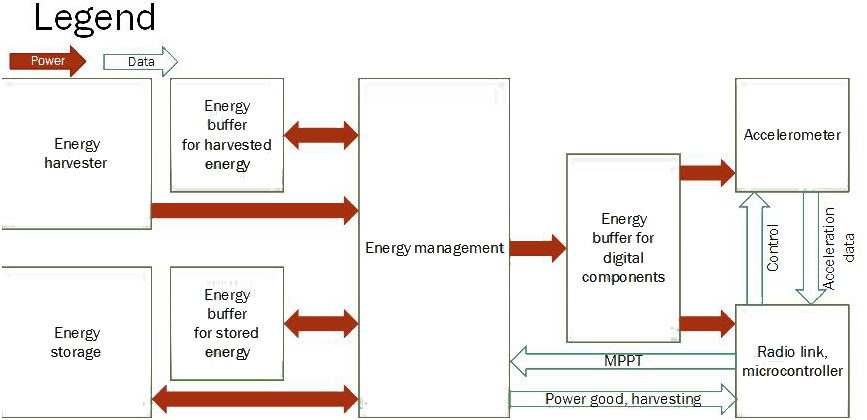
\includegraphics[height=6cm]{images/own_dwg/system_block_diagram.jpg}
\end{center}
\caption{\label{fiq:system_block_diagram} Block diagram of complete system. Harvested energy comes to system from top left, energy management system can charge storage when excess energy is available and use the stored energy when the harvested energy is insufficient for the system operation. On the right side is control logic and sensor. The experimental system has energy harvesting, energy storage and energy management sections, but control logic, radio comminication and sensing are outside the scope of the experimental work.}
\label{liitekuva}
\end{figure}

Energy harvester can use any suitable source presented in section \ref{sect:overview} for electrical energy. Energy management section rectifies AC voltage and buffers that rectified voltage on a capacitor. The energy storage can be a supercapacitor or a rechargeable battery. Both of these storage technologies can benefit from having a low equivalent series resistance (ESR) capacitor in parallel to supply peak currents. Energy management circuitry chooses whether to use harvested energy or stored energy and regulates the energy to voltage level compatible with the system. Digital components require their own local power buffer capacitors to supply high-frequency currents required by megahertz clocks onboard these circuits.

Microcontroller is used to manage the application layer of system. For example the microcontroller can send status updates over radio link more often if there is harvested energy available and reduce system power consumption when system is running on stored energy.

Next section presents details of expected power consumption and duty cycles for various components. A few components are selected to provide examples of suitable system power.

\subsection{Power requirements of a system} \label{sect:power_requirement}
The sensor system has in three distinct states. One is sleeping, conserving power as much as possible while the car is not moving.
Second state is measuring, when the radio connection is off but electronics are active and gathering data.
Third state is transmitting, when the data is relayed to a drive computer in the car.

Energy and power consumption are estimated by reviewing a few suitable components and their power requirements. 
Energy management is handled by a specialised integrated circuit (IC), LTC3331 \cite{Technology}.

Communication is handled by a Bluetooth-low energy (BLE) module, which contains a general-purpose microcontroller for application flow control.
We use BLE113 \cite{Bluegiga2013} which is such a module.

Finally there is an accelerometer which is used for gathering data out of the system, ADXL375 \cite{ADXLDatasheet}. ADXL375 is a low-power digital accelerometer with dynamic range of 200 g. Table \ref{power_consumption_table}  summarises the estimated power requirement of each subsection of system. System level voltage is selected to be 2.5 V, as that is lowest voltage which LTC3331 can supply and which allows all devices to function. Lowest possible voltage is selected to reduce the power draw.

\begin{table}[htb]
\caption{\label{power_consumption_table} Current and power consumption of system at different activity levels. Power is calculated from current by multiplying current with 2.5 V.}
\begin{center}
\fbox{
\begin{tabular}{l l r r}
\textbf{Device}		& \textbf{Sleep} 	& \textbf{Monitoring}	& \textbf{Communicating}\\ \hline
LTC3331			& 0.2 $\mu A$		& 80 $\mu A$ 		& 6 675 $\mu A$ 		\\ \hline
BLE113			& 0.9 $\mu A$ 		& 275 $\mu A$ 		& 26 000 $\mu A$	\\ \hline 
ADXL375			& 0.1 $\mu A$ 		& 140 $\mu A$ 		& 140 $\mu A$		\\ \hline 
\textbf{Total power}	& 3   $\mu W$		& 1 200 $\mu W$		& 82 000 $\mu W$	
\end{tabular}
}
\end{center}
\end{table}

Current consumption levels for BLE113 and ADXL375 are taken from the datasheets of the components. Battery manager power draw is estimated by calculating required power to supply the rest of the circuit at 80 \% efficiency. Power consumption is calculated from current draw with assumption that system voltage will be at constant 2.5 V.

Power consumption grows by orders of magnitude when the activity is stepped up to the next level. Therefore it is important to keep the system in sleep mode whenever possible, for example when the car is parked and wake up only periodically to check if the movement has started. Monitoring starts once the car is moving, and device will send brief pulses over the radio link when necessary.

When the power consumption is compared to values achieved in previous studies of energy harvesting presented in Section \ref{sect:state-of-art}, it can be seen that sleep current can be compensated by a reasonable harvester design. Powering constant monitoring would be a greater challenge, but within realm of feasibility. Providing power for continuous radio transmissions is not feasible even with the current state-of-the-art harvester designs. 

Next sections detail designs and preliminary analysis of the electromagnetic generator designs. The initial designs are then evaluated based on their ability to supply power at the required levels to the circuitry.

\subsection{Electromagnetic harvester design}
\subsubsection{Basics of the electromagnetical vibration harvester}
Electromagnetic harvesters utilise vibrations to move a magnet inside a coil. The movement of a magnet creates a changing magnetic field, which gets coupled to a coil. The coil opposes the change in the magnetic field by inducing electrical current in the device. A device could be built with a spring-loaded magnet to balance out the static acceleration of a tyre, an added benefit to spring loaded mechanism would be the utilisation of resonant frequency of the spring-mass system: as the system gets a shock, some of the energy would be in correct frequency range to make the magnet oscillate inside coil allowing generation of energy until next shock. The coil will also function as a damper to the system, so ideally no extra damping is required. Modern neodymium magnets do not lose their magnetisation by vibration, so a magnet can be reliable for a long time period. 

A theoretical design of linear generator (LG) was made. Most common generator designs use a rotating magnet inside coils to generate alternating current. As the mechanical apparatus for converting the linear accelerations inside the tyre to rotational movement would add to complexity and cost of the tyre, generator is designed to use the linear motion as the power source.

Basic principle of operation of LG is similar to traditional rotational generator. A moving magnet creates alternating magnetic field which is coupled to coiled conductors. The conductors oppose this change of magnetic field by inducing an electrical current across their ends. The design can have multiple phases and poles, where phases refer to parallel connected coils and poles refer to serially connected coils. Multiple phase designs can have lower resistive losses in wiring, as the resistive losses are proportional to square of the current. However paralleling phases requires separate rectification for each phase, which leads to increased rectification losses. Adding poles to design increases the output voltage and frequency, but having a small airgap between the coils and magnets becomes critical to maintain efficiency of the generator \cite{Cheng2008}. 

Energy harvester designs sometimes use several poles to increase the frequency of the power output. This increased frequency allows to use smaller energy storage components such as capacitors to keep the device powered until next cycle. The characteristics of the tyre make this point irrelevant, as energy is available once per revolution of the tire when generator contacts the ground and when the contact ends. Any energy storage device has to maintain power until the next cycle, and no increase of the frequency while generator is in contact can alleviate that. Therefore number of poles is minimised to reduce complexity. Pole number is selected as two, so there is one negative and one positive pole. Mechanical design can utilise resonant vibration to function as energy storage device instead of electrical or electronic storage.

First design decision was whether to use a design with a moving magnet or a moving coil. Moving coil designs tend to have lighter moving parts which is a very important feature in high-power designs where mass of the generator is large. On the other hand, moving coils require flying leads  \cite{Jacob2011},  which is a long-term reliability concern  \cite{Boldea1999}.  Boldea and Nasar \cite[p. 203]{Boldea1999a} conclude moving coil designs aren't practically interesting, so the design of the harvester is focused on moving magnet generator.

A rough model for designing the initial prototypes was done previously by Elmes \cite{Elmes2005}. As the work verified the model experimentally and found the model to be reasonably accurate, it was adapted to form basis of linear generator model. The model can account for most of the key design parameters. 

There are two different approaches to the generator structure. One is to have magnets inside, and coils on the outer rim of the generator. The other is to use ring magnets on the outer rim and have the coils on the inside. Both methods have their advantages: Having magnets on the outside allows larger and therefore stronger magnets and creates horizontal support for the magnets as they move along the shaft. Having coils on the outside increases wiring radius which results in greater power if other parameters are held equal. 

The height of the generator is constrained to avoid contact between tyre rim and generator. Initially the height of the generator was selected to be 35-40 mm to leave some margin while still being as tall as possible. Lower weight is desirable to avoid unbalancing the tyre, but there is no specific absolute maximum mass for the device. 

A method to counter the centripetal acceleration is needed to keep the magnet on the centre of the generator. Ideally, such method would always balance the magnet in the middle of generator against any external constant force, but active control is not achievable without adding to complexity and power consumption of the generator itself. Passive negative feedback method has to be used instead. 

Springs are often chosen to balance the magnets, but the centripetal acceleration grows exponentially with the speed of the car. Therefore any linear spring would be usable only for very limited range of speeds, the problem could be alleviated with non-linear conical springs which have the added benefit of compressing into very small height.

Another approach would be to use two additional magnets fixed to top and bottom of the generator in repulsive configuration. Force between magnets is inversely proportional to fourth power of the distance \cite{Amrani2015}, which leads to a strong negative feedback on the position of the magnet. Tornincasa et al. \cite{Tornincasa2012} proposed one such design, shown in Figure \ref{lgm}.

\begin{figure}[htb]
\begin{center}
\includegraphics[height=4cm]{images/cited/lgm}
\end{center}
\caption{A magnetically balanced linear generator by Tornincasa et al. \cite{Tornincasa2012}}.
\label{lgm}
\end{figure}

Magnetic floating is an attractive solution, as magnets can be thin and they do not wear out with ageing. On the other hand, any imbalance in the magnets can result in torque which causes increased friction as shown in Figure \ref{fig:lg_torgue}. This issue is further aggravated in designs where shape of the generator shaft is not a smooth cylinder. Therefore the design should have reasonably smooth and low-friction material on the inner shaft to minimise frictional losses.

\begin{figure}[htb]
\begin{center}
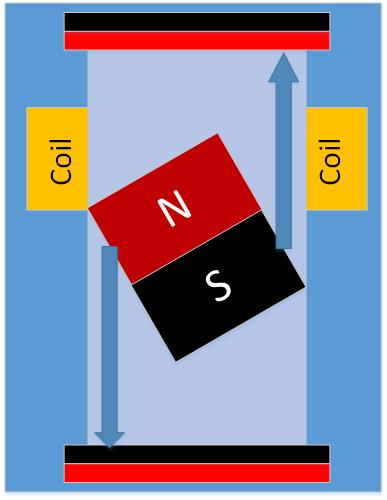
\includegraphics[height=6cm]{images/own_dwg/generator_torgue}
\end{center}
\caption{Angle in magnet causes torque which results in increased friction}.
\label{fig:lg_torgue}
\end{figure}



\subsubsection{Analytical model of the electromagnetical vibration harvester}
A common starting point for analysis of linear generator is to model the mechanical domain as Mass-Spring-Dampener system decipted in Figure \ref{MSD}. A mass "floats" in the system, a spring balances the mass towards the centre and a damper represents frictional forces opposing any movement of the mass. 

\begin{figure}[htb]
\begin{center}
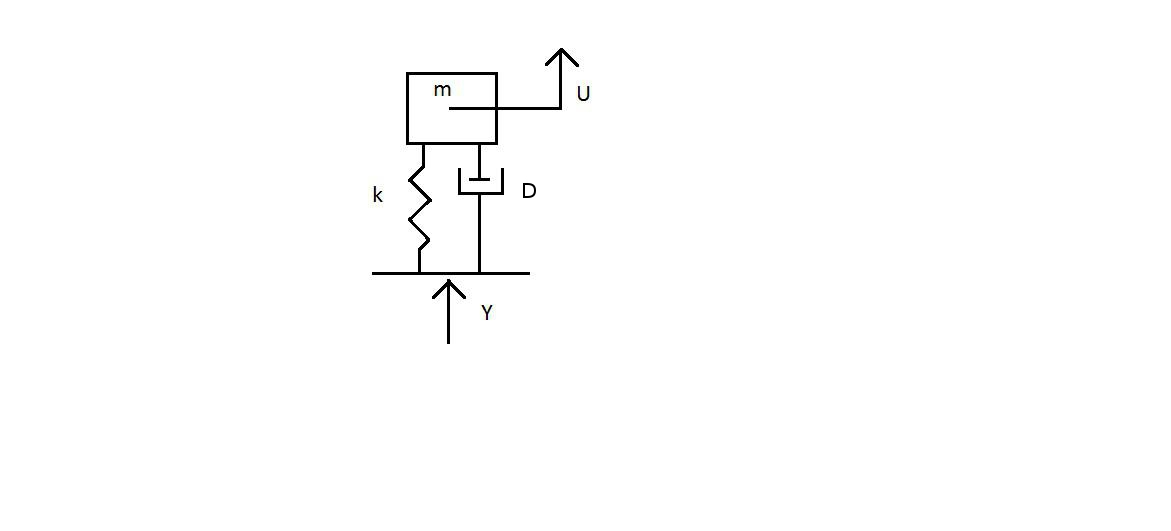
\includegraphics[height=6cm]{images/own_dwg/MSD.jpg}
\end{center}
\caption{\label{MSD} Mass-spring-damper system.}
\end{figure}

Mathematical representation of this system is given in Equation \eqrefeq:{MSD_basic}. Input Y is the force applied to the base of system, output U is the position of mass block relative to "zero". Zero is usually set to the point where the mass settles when no input, including gravity, is applied to the system. Parameters m, D, and k are mass, damping constant and spring constant of system, respectively. Input-output-equation in time domain can be written as: 

\begin{equation}\label{eq:MSD_basic}
  m \cdot \ddot{U}(t) + D \cdot \dot{U}(t) + k \cdot U(t) = Y(t). 
\end{equation}

As the force $ Y(t) $ is defined as $ Y(t) = m \cdot a(t) $, and the acceleration $ a(t)$ can be considered constant regardless of any reasonable mass $ m $ of system, equation \eqref{eq:MSD_basic} can be written as:

\begin{equation}\label{eq:MSD_acceleration}
 \ddot{U}(t) + \frac{D \cdot \dot{U}(t)}{m} + \frac{k \cdot U(t)}{m} = a(t). 
\end{equation}

This form is more convenient for analysis, as the acceleration measurements from previous research are available and they represent real-world values. Mass $m$ can be considered constant, as the system does not exchange matter with surrounding environment. As magnetic suspension was selected, the parameter $k$ cannot be considered as a constant, but rather a function of mass position $k(U)$. Centripetal force can be considered as a constant DC-component of function $Y(t)$, and is not included in analysis of function $k(U)$. According to D. Amrani \cite{Amrani2015} force between two magnets can be approximated as

\begin{equation}\label{eq:magnetic_force}
  F(x) = \frac{3 \mu_0 m_1 m_2}{2 \pi} \cdot \frac{1}{x^4},
\end{equation}

where $F(x)$ is force as a function of distance $x$ between magnets, $\mu_0$ is the permeability of vacuum, $ m_1 $ and $ m_2 $ are magnetic dipole moments of magnets under examination. This equation is only valid when $x >> h$, where $h$ is thickness of the magnet. As two magnets are used to suspend the rotor magnet, total force acting on mass becomes 

\begin{equation}\label{eq:magnetic_force_middle}
  F(x) = \frac{3 \mu_0 m_r m_l}{2 \pi} \cdot \frac{1}{(x_0+x)^4} - \frac{3 \mu_0 m_r m_u}{2 \pi} \cdot \frac{1}{(x_0-x)^4},
\end{equation}

where $m_l, m_u, m_r$ are magnetic dipole moments of lower suspending magnet, upper suspending magnet, and rotor magnet. $x_0$ is the distance to middle point of generator and $x$ is the displacement of rotor magnet from aforementioned middle point, positive direction being upwards. Figure \ref{fig:lg} shows the system.

\begin{figure}[htb]
\begin{center}
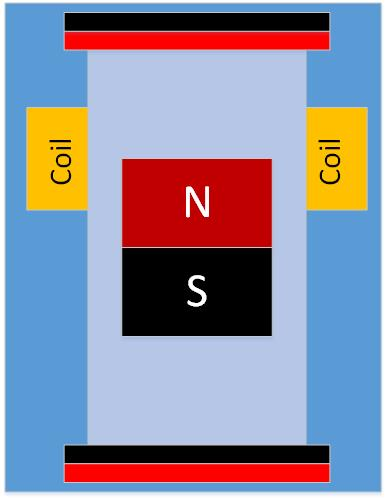
\includegraphics[height=6cm]{images/own_dwg/generator}
\end{center}
\caption{Linear generator with rotor magnet balanced by endstop magnets}.
\label{fig:lg}
\end{figure}

However, the Equation \eqref{eq:magnetic_force_middle} is very inaccurate for magnets where diameter is large compared to thickness of magnet, and the problems are compounded when distance between magnets is small. Therefore final design was optimised using finite element analysis (FEA) for determining $k(U)$. 

Damping parameter $D$ is likewise a function of electromagnetic force acting on the magnet, friction between the magnet and the stator and pneumatic damping caused by compression of air in the generator. Tornincasa et al. \cite{Tornincasa2012} divided this damping parameter into three distinct terms to account for these different physical phenomena in damping. Let us call them $D_{emf}, D_{friction},$ and $D_{air}$, respectively. $D_{emf}$ represents power extracted from the system into electrical current, it can be written as:

\begin{equation}\label{eq:d_emd}
  D_{emf} = BIlsin(\phi),
\end{equation}

where $B$ is magnetic field affecting coil (presumed constant), $I$ is current through wire depending on load and generator properties, $l$ is total length of wire in coil and $\phi$ is angle between coil and magnetic field, presumed to be 90 \degree. Assuming the load impedance is the complex conjugate of coil impedance for maximum power harvesting, we can substitute the $I$ with equations \eqref{eq:emf} and \eqref{eq:gen_simple_current}, which results in: 

\begin{equation}
  D_{emf} = B \frac{\varepsilon}{2 \cdot Re(Z_{generator})} l sin(90 \degree),
\end{equation}

where $Z_{generator}$ is the impedance of generator. As the load impedance is complex conjugate of generator impedance, their series connection has only real (purely resistive) component. This assumption fails on real-world application with non-linear rectification and DC/DC conversion, but it can be used as a basis for analytical examination of the generator. As $\varepsilon$ can be substituted with \eqref{eq:emf}, we obtain:

\begin{equation}\label{eq:d_emf_with_epsilon}
  D_{emf} = B \frac{-N \frac{d \Phi_{B}}{d t}}{2 \cdot Re(Z_{generator})} l sin(90 \degree),
\end{equation}

The relationship between $N \Phi_{B}$ and $Re(Z_{generator})$ can be further studied by writing: 

\begin{equation}\label{eq:phiB_substitution}
  \Phi_{B} = \iint_{\Sigma (t)} B(r, t) \,dA,
\end{equation}

where $ \iint_{\Sigma (t)} $ signifies possibility of the loop area changing over time and $\,dA$ is an element of the surface area. If we assume the coil to be a perfect tightly wound circle which does not deform over time, we can write the relationship between number of turns in the coil, area of the coil, and resistance of the coil as:

\begin{equation}\label{eq:nA_R}
  R = N 2\pi A \rho_{wire},
\end{equation}

where $\rho_{wire}$ is the resistivity of coil wire. Substituting Equations \eqref{eq:nA_R} and \eqref{eq:phiB_substitution} into Equation \eqref{eq:d_emf_with_epsilon} we finally obtain reasonably accurate expression for $D_{emf}$ which accounts for all the design parameters affecting it:
\begin{equation}\label{eq:d_emf_complete}
  D_{emf} = B \frac{-N \frac{d [\iint B(r, t) \,dA]}{d t}}{2 \cdot N 2\pi A \rho_{wire}} l sin(90 \degree).
\end{equation}

A few observations can be made from this equation: first, the magnetic field strength $B$ and its derivate in respect to time increase the $D_{emf}$ which signifies the electrically extracted useful power. Therefore it makes sense to use as strong magnets as possible as long as other parameters aren't adversely affected. Second, both the number of turns $N$ and the loop area $A$ are in nominator and denominator, which means they should be optimised to find the best applicable values. Third, resistivity of wire limits the power that can be extracted, so intuition would lead to minimising the wire resistance. In practise the wire resistivity can be decreased by increasing the wire diameter, which in turn leads to lower number of turns in same the volume and mass of the coil. Therefore, also wire diameter and material should be optimised to find desirable compromise in the generator design. 

Next we examine $D_{friction}$ in detail. Friction is modelled as Coulomb friction:
\begin{equation}\label{eq:Coulomb_friction}
  F_s = \mu_sN,
  F_k = \mu_kN,
\end{equation}

where $F_s $ and $ F_k $ are static and kinetic friction forces opposing movement, $\mu_s$ and $\mu_k$ are friction coefficients in static and kinetic situations and $N$ is normal force along X- or Y- axis. Normal forces are estimated by using the existing acceleration data and calculated mass of magnet. Coefficients of friction are looked up from the supplier of stator material. Transfer between static and kinetic models is assumed to be a step, if velocity of magnet is 0 along Z-axis, $\mu_s$ is used, $\mu_k$ otherwise.

Finally, there is pneumatic damping of the system, $D_{air}$. In a closed tube, the central magnet can be thought of as a piston dividing the generator into two chambers. If there is an insignificant airflow between chambers, any force caused by pressure deltas between chambers act as a spring. However, some airflow is to be expected due to the clearance between the magnet and the stator. Tornincasa et al. \cite{Tornincasa2012} modelled this effect by adding a virtual centrepoint for the pneumatic spring. This centre moves through a virtual damper which models the airflow between the chambers. End result is that the pneumatic spring takes some energy from movement, and the energy stored into pneumatic spring is dissipated as the centre moves until potential energy stored in the spring is zero. 

The force from pressure differential is:

\begin{equation}
  F_{\delta p} = \frac{\pi d^2}{4}(p_{lower}-p_{upper}),
\end{equation}

where $d$ is diameter of magnet and $p_{lower}-p_{upper}$ are pressures in chambers. Pressures can be estimated from ideal gas law:

\begin{equation}
  pV = NRT
\end{equation}
where $p$ is pressure, $V$ is volume, $N$ is amount, $R$ is ideal gas constant and $T$ is temperature. Temperature is assumed to be constant. Initial pressure is assumed to be same as tyre pressure and magnet is assumed to be exactly in midpoint at start. Change of volume can be calculated from change of height caused by movement of the magnet. 

Mass flow between sections can be estimated with equation given by Fox et al. \cite{Fox2008}:

\begin{equation}
  \dot{m}_{1 \rightarrow 2} = \frac{\rho \pi d {\delta_r}^3}{12\mu h}(p_1-p_2),
\end{equation}

where $\rho$ is air density, $\delta_r$ is radial clearance, $\mu$ is dynamic viscosity and $h$ is the height of magnet. \cite{Tornincasa2012}

There is also frictional dissipative force as the air passes along the edges of the cylinder. This frictional force has magnitude of: 

\begin{equation}
  F = \mu \cdot \rho \cdot \frac{\pi d h \dot{z}}{\delta} \cite{Medhat2008}. 
\end{equation}

Analytical expressions for the equations governing the mechanical movement of magnet inside generator have now been identified. Some of the non-linear functions are hard to solve analytically, therefore experimental and FEA methods are used for creating approximations for these functions.

The analytical effect of these parameters is summarised in Table \ref{parameters_of_lg}

\begin{table}[htb]
\caption{\label{parameters_of_lg} Effect of the parameters of the generator}
\begin{center}
\fbox{
\begin{tabular}{l l l}
\textbf{Parameter}          & \textbf{Increasing} 		& \textbf{Decreasing}	\\ \hline
\(\displaystyle N_{turns} \)& Higher voltage		& Smaller size, less wiring resistance 		\\ \hline
\(\displaystyle N_{pole} \) & Increased frequency		& Decreased frequency	\\ \hline
\(\displaystyle l_{pole} \) & More space for wiring 	& Higher voltage, smaller size	\\ \hline
\(\displaystyle A_{loop} \) & More power			& Smaller length of wiring 	\\ \hline
B                           & Increased power 	        & Smaller magnets 		\\ \hline
\(\displaystyle r_{wire}\)  & Decreased wiring resistance 	& More turns in same space 	\\ \hline
\(\displaystyle \delta_{r} \) & Stronger side walls		& Increased efficiency 
\end{tabular}
}
\end{center}
\end{table}

This section has given analytical expressions on forces acting on the magnet. With the expressions known, next section presents simulation and experimental methods for evaluating the effects of these expressions.

\subsubsection{Experimental and FEA modeling of the electromagnetic harvester}
Some parameters of the harvester are difficult to solve analytically. These parameters are estimated using experimental and FEA methods. First one of these difficult interactions is the magnetic force between rotor magnet and balancing magnets. A magnetics FEA software FEMM \cite{Meeker2013} was used to create an axisymmetric model of magnets in the generator. Figure \ref{femm_forces} shows the used model. Ths model has two opposing magnets made of N40-neodymium alloy configured to repel an identical rotor magnet. The magnets have a height of 2.5 mm and diameter of 11 mm, walls of generator are modelled as air. The generator has total height of 25 mm, leaving the rotor magnet 17.5 mm room for movement inside the generator.

Weighted stress tensor integration over rotor magnet volume as implemented by FEMM was used to determine FEA value for the net magnetic force acting on the rotor magnet. A LUA script was used to move the rotor magnet from the bottom of the generator to the top in 0.1 mm increments and values obtained from the analysis were exported as CSV data for plotting in a spreadsheet software as well as to create a lookup-table for MATLAB/SIMULINK simulation. Figure \ref{femm_forces} shows the force on the magnet, positive force meaning force towards the upper magnet and zero height being at in the middle of the cylider. The centrifugal force acting on magnet was also calculated at various speeds for reference, assuming weight of the magnet is 1,67 g and radius to the bottom of generator is 275 mm.

\begin{figure}[htb]
  \begin{center}
  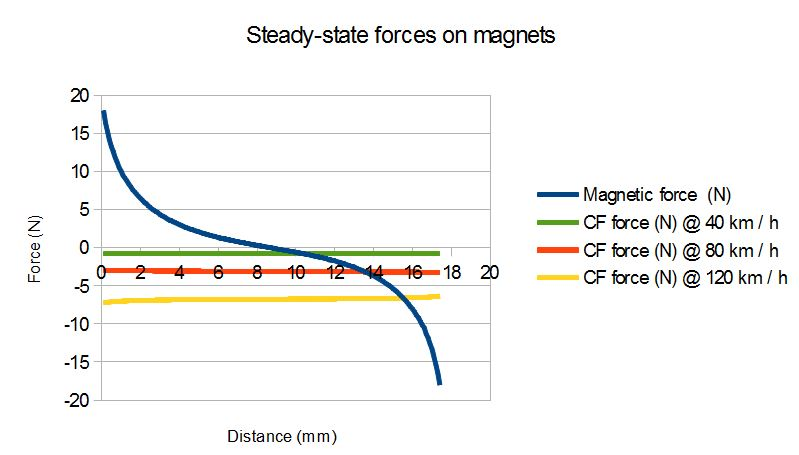
\includegraphics[height=6cm]{images/own_dwg/femm_fvsd_dualmagnet.jpg}
  \end{center}
  \caption{\label{femm_forces} Steady-state forces acting on magnet. The magnetic force will counteract centrifugal force at 2 mm, 5 mm and 7 mm displacement from center for speeds of 40, 80 and 120 km / h respectively.}
\end{figure}

It can be seen that net force on rotor magnet is dominated by the magnetic forces at lower speeds. Centrifugal force on magnet becomes significant at higher speeds, and at120 km/h speed the rotor magnet can impact the bottom assuming 30 mm displacement as estimated in Figure \ref{fig:deformation} in Section \ref{sect:tyre_environment}. Second use for this FEA analysis was to create a look-up table for flux linkage into the coils of the generator. The methodology was similar to determining the forces affecting the rotor magnet: a LUA script was ran to sweep the possible magnet positions, and the look-up table of flux linkage into coils was created. For the purposes of analysis, difference of flux linkage was calculated between each point. The change of flux linkage is a very important parameter, as the power generated is proportional to $\frac{d \Phi_{B}}{d t}$. 

\begin{figure}[htb]
\begin{center}
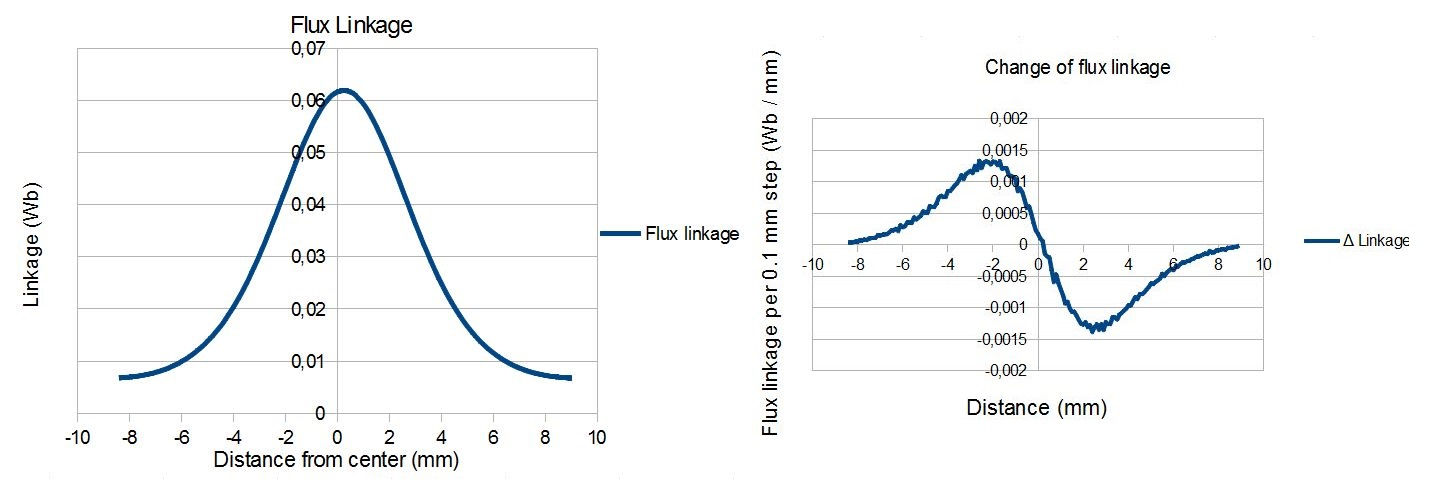
\includegraphics[height=6cm]{images/own_dwg/femm_flux_dualmagnet.jpg}
\end{center}
\caption{\label{fig:femm_linkage} Flux linkage and rate of change in 0.1 mm steps in generator. Derivative of flux linkage in respect to position is largest near 2 - 3 mm displacement from the centre of the coil.}
\end{figure}

Based on these results, a magnet moving at the speed of $0.1 mm / s $ would induce voltage of up to $1.5 mV$ in each winding of the coil.

\begin{comment}

A prototype generator was built to test the concept feasibility and identify any practical issues in the generator construction. Generator was machined out of 21mm diameter nylon tubing with 12 mm inner diameter. A groove was machined on the outer diameter to hold the coiling in place. Inner diameter of the groove was 14 mm and height 3 mm. 0.1 mm diameter wire was used to build the coil. To determine the number of turns in coil, coil resistance was measured to determine the length of wire and number of turn was calculated using known length of loop turn and total length of wire. Coil resistance was 42 ohms as the resistance of wire is approximately 2.2 ohms / meter the total length is approximately 19 meters. As one loop has length of 44 mm, coil had roughly 400 turns. 

The prototype was connected on a  Brüel \& Kjær shaker type 4905 and driven using  Brüel \& Kjær power amplifier type 2707. Input signal was generated using NI-USB6218 DAQ and output was measured directly from leads of the generator. Vertical displacement of generator was limited to $7.5 mm$. Output signal was a sine wave with amplitude of $\pm$ 5 volts, which was amplified by gain of 8 above frequencies of 30 Hz. At lower frequencies the gain was limited to stay within allowed displacement. Measured graphs are shown in figure \ref{fiq:lg_proto_results}.

\begin{figure}[h]
\begin{center}
  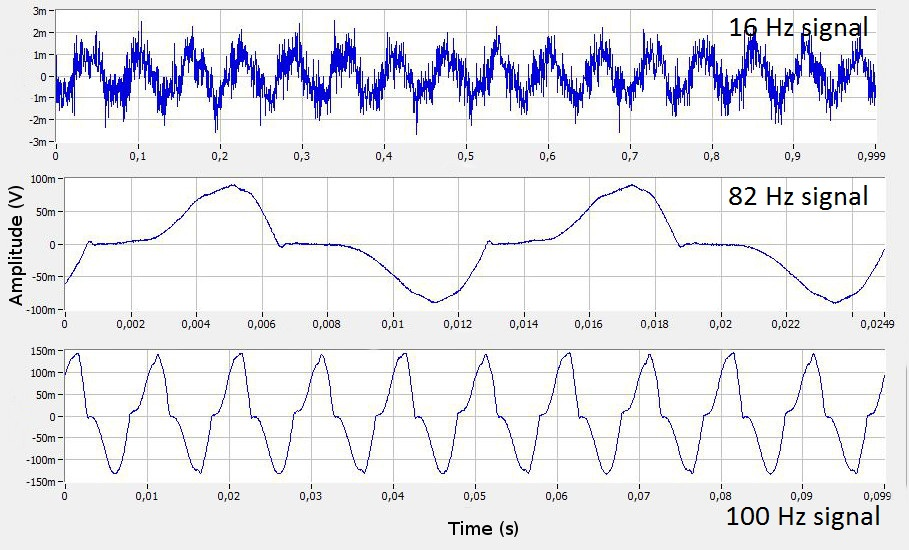
\includegraphics[height=8cm]{images/own_measurement/lg_proto.jpg}
  \end{center}
  \caption{\label{fiq:lg_proto_results} Measured open-loop voltage outputs at various frequencies}
\end{figure}

At low frequencies the magnets do not overcome friction and only measurement noise is present in signal. In addition to white noise in measurement there is a sine wave with amplitude of hew millivolts which correlates with the excitation signal. The measurement noise is insignificant when compared to signal generated my moving magnet. 

At low frequencies the magnet cannot overcome the friction and only noise is present in measurement. Around 82 Hz the magnet could move inside shaft, producing peaks with roughly 100 $mV$ peaks. The magnet stops in between of the peaks which is seen as valleys of no voltage being produced. 

Peak voltages of roughly 150 mV were achieved at 100 Hz. The magnet is in almost constant motion, a brief stop can be seen when the magnet changes direction. 

While 150 mV is notably less than the few volts predicted by Simulink model, the basic operation principles was validated by quick experiment. The difference in output voltage is probably due to imprecise construction in prototype harvester. As the concept was proven, the design of generator was finalised. Next section details the exact construction of final electromagnetic generator. 

\subsubsection{Mechanical design of electromagnetic harvester}\label{sect:emh_design}
Few practical issues became evident during construction of prototype generator. Machining grooves to plastic tubes caused warping to tube, which prevented magnet from moving inside coils. Shallow grooves would not keep the coils in place, as wires being loose would fall off the groove. The tube did not offer any reasonable mount point for a printed circuit board. 

Issues with grooves were solved by selecting a tube with minimal wall thickness and using separators to contain the coil. A separate housing was designed to hold the tube and to offer mounting points for the circuit board. 

A layered design was made for the harvester. On the bottom is a solid square with 35 * 35 mm sides and holes for screws on corners. Next layer has a hole for the bottom magnet, third layer has hole for the tube. Tube has a spacer in middle to hold the coil below midpoint. Top half of harvester is symmetrical to bottom. 

\end{comment}

\subsection{Piezoelectric harvester design}
\subsubsection{Basics of the piezoelectric energy harvesting }
This section details experimental identification of properties of the piezoelectric element used in the harvester. A testbed with an impactor providing excitation was used to generate experimental values for power output and voltage at various operating conditions for the piezo element.

Thunder\textsuperscript{(TM)} piezos have been used in previous studies of piezoelectric harvesting and they have produced promising results \cite{Manla2009}, so they were selected as the piezoelectric element for this thesis.

Series of tests were ran to determine the characteristics of piezoelectric power generation under impacts. Mossi et al \cite{Mossi} have produced a recommended test process for Thunder piezoelectric actuators shown in Figure \ref{fiq:thunder_eval}.

\begin{figure}[htb]
  \begin{center}
  \includegraphics[height=6cm]{images/cited/mossi}
  \end{center}
  \caption{Recommended evaluation platform for Thunder piezos \cite{Mossi}.}
  \label{fiq:thunder_eval}
\end{figure}

This setup was replicated using a solenoid actuator as an impact force generator, a precision scale as load cell to measure the impact force and an oscilloscope to view the output waveforms. An eraser was cut to shape to act as preload bellow to spread the impact over larger surface area of piezoelement. Displacement was not measured. The test setup is shown in Figure \ref{fiq:piezo_impact}. An electronics prototyping platform, "breadboard", was used to house test the electronics including a resistive ladder and an Arduino to trigger the solenoid at adjustable duty cycles. Load force was controlled by setting the stroke length of the solenoid shaft and fine tuned by adjusting the voltage over the solenoid. 

\begin{figure}[htb]
  \begin{center}
  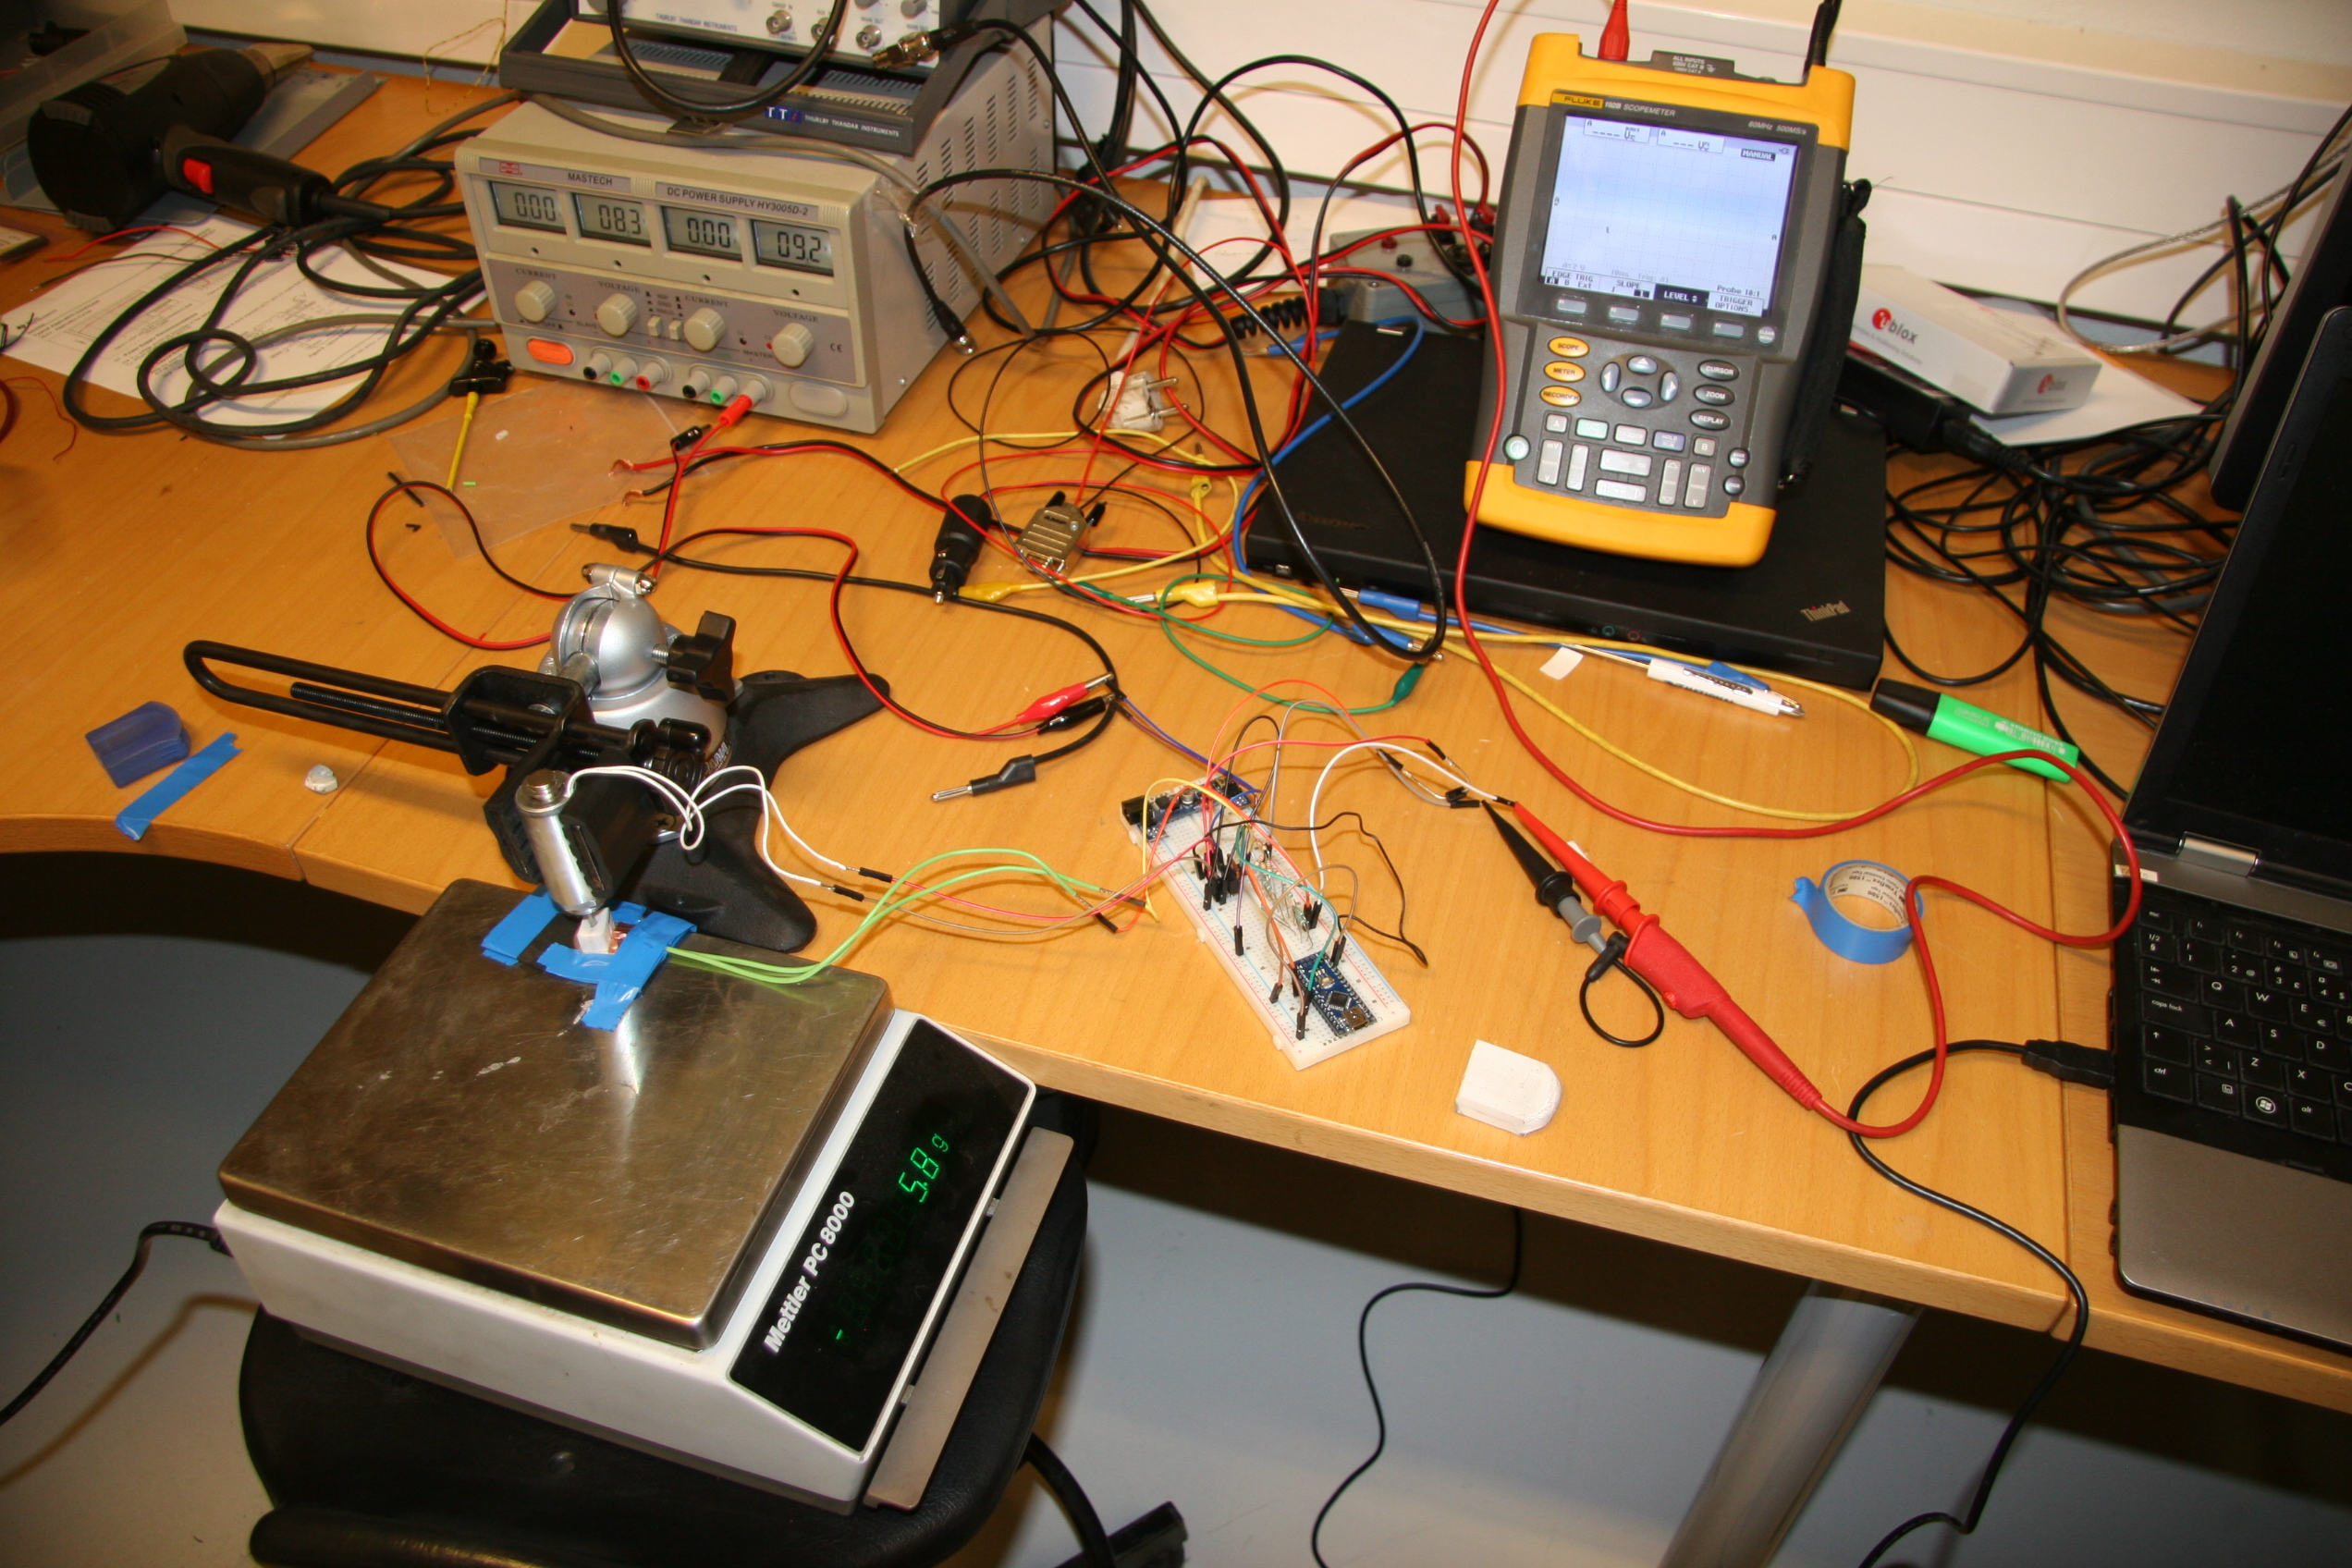
\includegraphics[height=6cm]{images/own_pic/piezo_test}
  \end{center}
  \caption{Test platform for piezo characteristics.}
  \label{fiq:piezo_impact}
\end{figure}

The measurement results are shown in Figure \ref{fiq:piezo_measurement_chart}. Output voltage scales with square of impact force, which is sensible as the work done can be expressed as $W = F \cdot d$, where $W$ is work, $F$ is force and $d$ is a distance the force acts on an object. As the displacement of the piezoelement grows with the applied force, total work and therefore energy grows with the both terms. 

\begin{figure}[htb]
  \begin{center}
  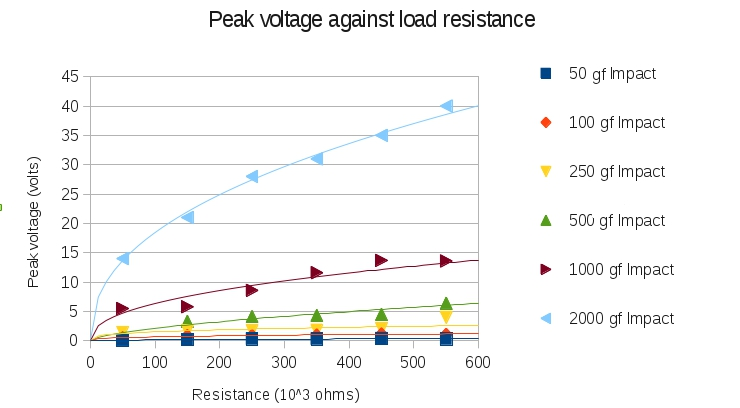
\includegraphics[height=6cm]{images/own_measurement/piezo_measurements}
  \end{center}
  \caption{Measured output voltage at different loads and impact forces.}
  \label{fiq:piezo_measurement_chart}
\end{figure}

Peak voltage grows with the load resistance. This is in agreement with both the voltage source and the current source models, as the capacitor starts to discharge through the load resistance instantly when a voltage is applied over it. The relationship between voltage and load resistance seems to be logarithmic, which would be in an agreement with the logarithmic discharge curve of the capacitor-resistor system. Peak voltages were read out from a digital display and they can be considered reasonably accurate.

The time constants for a voltage halving were graphically measured from oscilloscope waveforms, and this data was used to calculate the capacitance of TH-5C. These measurements are a lot less accurate, as readouts from an oscilloscope screen have resolution of approximately half of the line division, making the accuracy of measurements at $\pm 2.5 ms$. These results are shown in Figure \ref{fig:piezo_time_capacitance}

\begin{figure}[htb]
  \begin{center}
  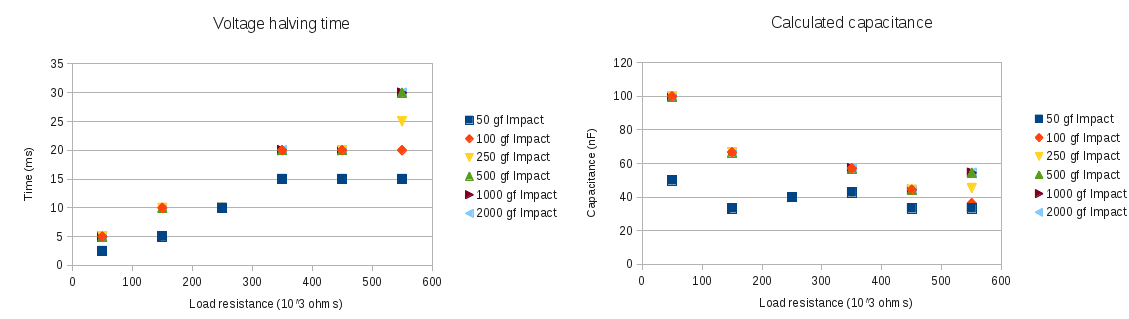
\includegraphics[height=4cm]{images/own_measurement/piezo_capacitance}
  \end{center}
  \caption{Measured half-time of system and the calculated capacitance of piezo.}
  \label{fig:piezo_time_capacitance}
\end{figure}

The half-time data can be used to calculate the capacitance of piezo using the RC-time constant of circuit:

\begin{equation}
  C=\frac{t}{-ln(\frac{1}{2})R} 
\end{equation}

TH-5C provides a value of 39 nF as the capacitance, while these calculated values are notably higher and rise with the loading of the piezoelement. Most likely explanation of this observation is the mechanical response time of system: the solenoid plunger will take some milliseconds to reach new force equilibrium, and this effect becomes more pronounced at smaller time constants of the RC-system. Using the known voltage and capacitance energy and peak power in impact can be determined:
 
\begin{equation}
   E = \frac{1}{2}V^2C
\end{equation}

\begin{equation}
   P_{peak} = \frac{V^2}{R}
\end{equation}
 
The calculations are shown in  Figure \ref{fig:piezo_power_energy}. As these calculations are based on inaccurately measured time, they should not be used as reference for any further calculations. However, trends can be seen in these values. 
 
 Interestingly the peak work done by the piezoelement to the resistor seems to be almost constant on all load levels. This is probably a consequence of the logarithmic voltage-load relationship described earlier in this section. There is a possibly significant result based on these findings: total energy obtainable from harvester grows with the load resistance. However, this is applicable only for a resistive load under impact-based energy generation.
 
 \begin{figure}[htb]
  \begin{center}
  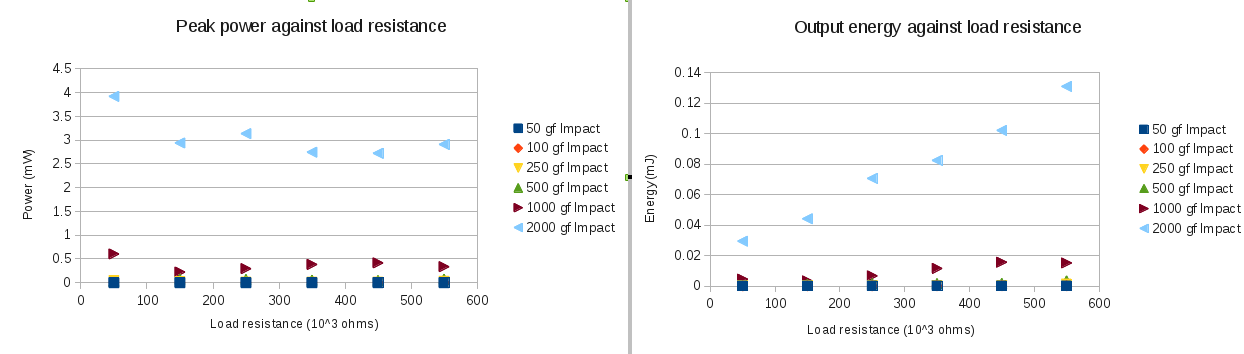
\includegraphics[height=4cm]{images/own_measurement/piezo_power}
  \end{center}
  \caption{Calculated piezo power and energy output}
  \label{fig:piezo_power_energy}
\end{figure}

Based on these results, an electrical equivalent model of the circuit was designed. The model is shown in Figure \ref{fig:piezo_ltspice_equivalent}. Model has two parallel current sources, one to simulate impact of the plunger on the piezoelement and other to simulate the release of the impact. Capacitance in parallel is set to 39 nF as given in the datasheet, load resistance is parametricised to step through the experimental values.

Model was tuned by first calculating the total current transfer to reach the open circuit voltage over capacitor. Then maximum current of current sources was matched to the peak voltage over highest load.
The simulated data is plotted Figure \ref{fiq:piezo_simulation_experimental}.

 \begin{figure}[htb]
  \begin{center}
  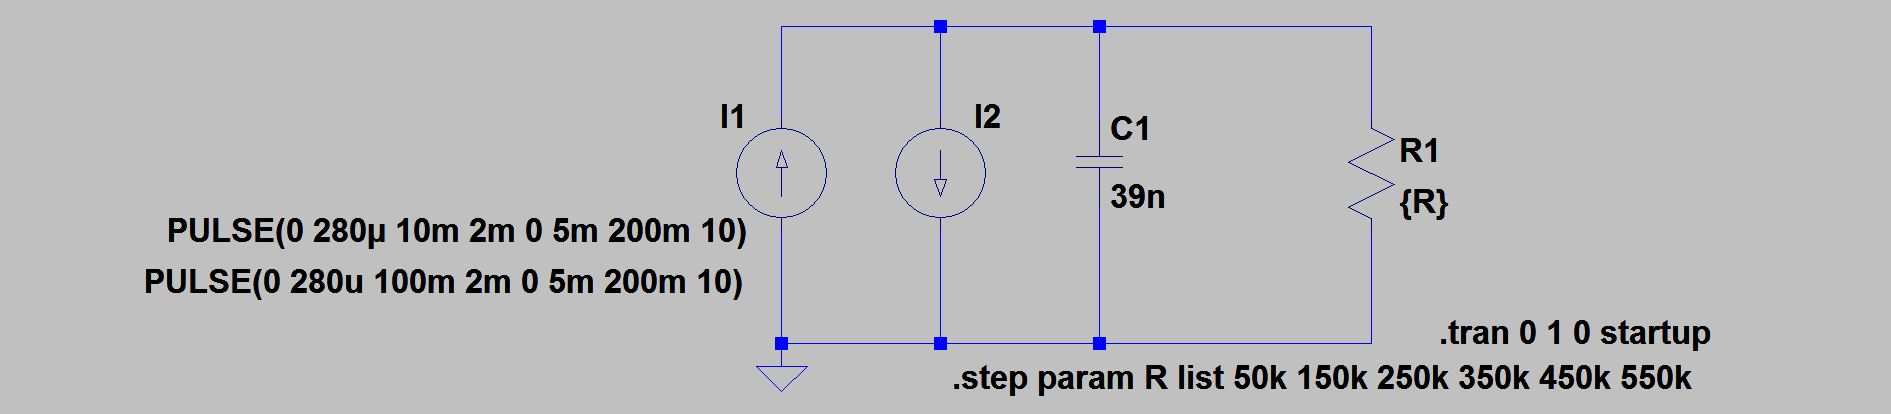
\includegraphics[height=6cm]{images/own_dwg/ltspice_piezo}
  \end{center}
  \caption{Equivalent model of piezo in LTSpice simulator}
  \label{fig:piezo_ltspice_equivalent}
\end{figure}

 \begin{figure}[htb]
  \begin{center}
  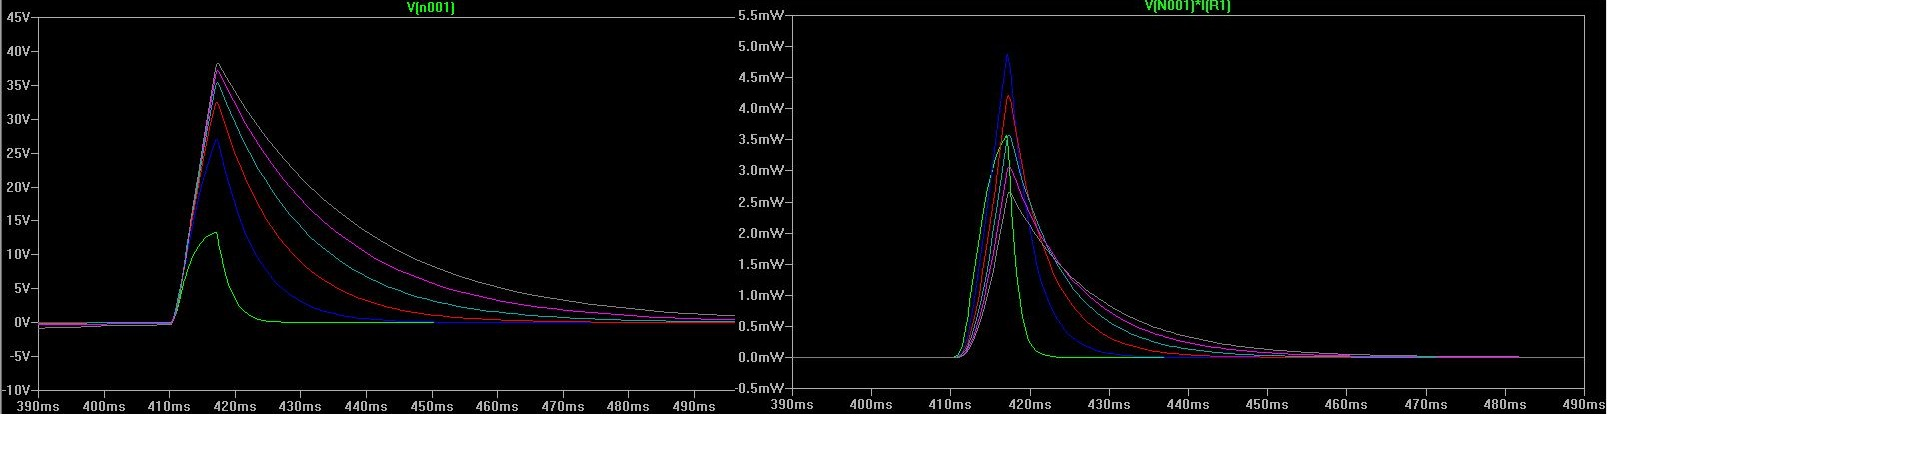
\includegraphics[height=8cm]{images/own_dwg/ltspice_piezo_simulation}
  \end{center}
  \caption{Simulated piezoelement output voltage and power waveforms. Loads are stepped through list to match experimental values at 2000 gf impact force. Black: 50k; Blue: 150k; Red: 250k; Green: 350k; Pink: 450k; Gray: 550k}
  \label{fiq:piezo_simulation_experimental}
\end{figure}

The experimental and simulated data are not in an agreement. While maximum and minimum load voltage and power are close to estimated values, this is by design as the model is tuned to these measurements. Problems occur in interpolating the results, as output voltages are notably higher than measured values. This provides a result which sets the maximum power load near the value which provides output voltage of half of the open loop voltage. This is especially interesting as LTC3331 datasheet \cite{Technology} suggests to set the circuit to track the load at this same half-point of open loop voltage. Both LTC3331 and LTSpice are made by Linear Technology, so independent verification of this result would be necessary. 

\subsection{Electronic design} \label{sect:electronic_design}
\subsubsection{Simulation of the circuit}
As the focus of work is on energy harvesting, only analog sections related to energy harvesting are simulated. Digital loads are simulated as current sinks. This section details the simulation model used to validate the design of circuitry.

The analog sections of circuit were simulated using LTSpice IV \cite{ltspice}. Microcontroller, radio link and accelerometer were simulated as resistive load. Battery was modelled as a voltage source with high-value capacitor and low-value resistor in series. Piezoelectric harvesting was modelled both as high-voltage source with capacitor in series, and as a current source with capacitor in parallel. Electromagnetic harvesting was modelled as low-impedance low-voltage source. 

LTC3331 presents an interesting opportunity for maximum power point tracking (MPPT). While the impedance of individual components cannot be tuned in real-time, the microcontroller can determine the rotation frequency of the tyre from the accelerometer readings and determine the maximum power point. LTC3331 can adjust the target voltage for the energy storage buffer capacitor, which enables MPPT-control of system.

The simulation model is shown in Figure \ref{fig:ltspice_sim}. Connections were adjusted as needed to generate simulation data for different purposes, such as measuring energy efficiency, transient response, MPPT etc.

\begin{figure}[htb]
\begin{center}
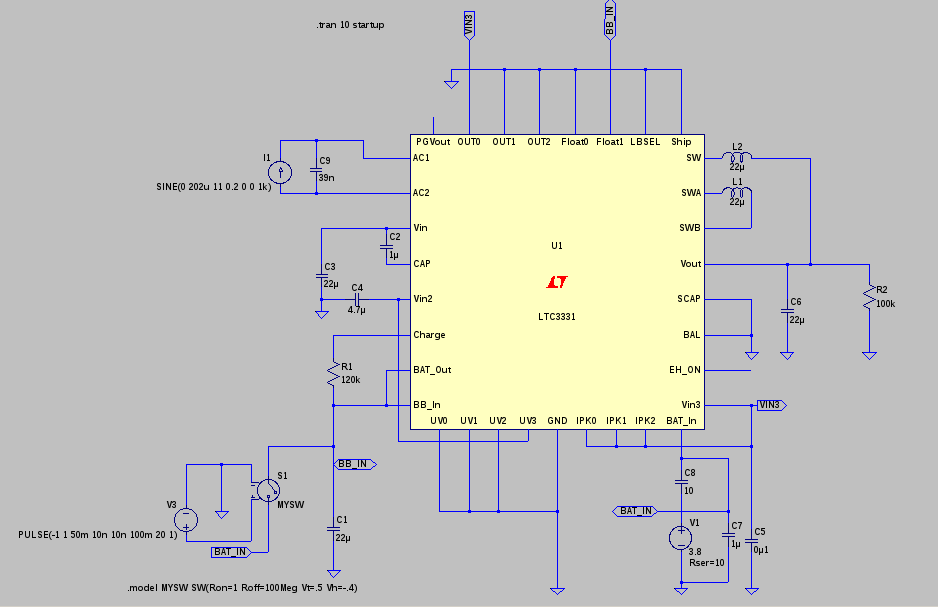
\includegraphics[height=12cm]{images/own_dwg/ltspice_ltc3331.jpg}
\end{center}
\caption{\label{fig:ltspice_sim} LTSpice \cite{ltspice} simulation of electrical circuit}
\end{figure}

The simulation model was used to validate the basic operation of the circuit, circuit operates as the datasheet specified. As the basic operation of circuit has been validated, next step was to design the detailed schematic for the circuit. The next section details schematic design of the circuit, starting from top-level diagram and connections between blocks, followed by detailed design of each subblock. 

\subsubsection{Schematic design}
The schematic is a logical representation of the components and how they connect to each other. The schematic is designed in accordance with the datasheets, reference designs and application notes of the main circuit components. This section details the schematic diagram of the circuit.

As the design operates in a high-vibration environment with wide temperature variations, special care was used to select components which have well-defined temperature and mechanical characteristics. 

Since the circuit is a low-power design, careful attention was paid to parasitic properties and non-ideal behaviour of components. For example electrolytic capacitor can have leakage current of several microamperes \cite{Both2001}, which is in the same order of magnitude as the targeted sleep current consumption of system. Likewise any signalling current was kept at minimum. 

Another important point of view is the modularity and testability of the circuit. All critical lines have provision for testing and debugging for development and verification of the circuit functionality. Figure \ref{fig:circuit_blocklevel} shows the interconnections in system, drawn in KiCAD \cite{KiCAD}.  The power supply can be cut off to separate sections of circuit for current measurement as needed. This has additional benefit of leaving places for power supply filtering components in case some section of circuit emits electrical noise through power supply lines.

\begin{figure}
    \centering
    \def\svgwidth{\columnwidth}
    \input{images/own_dwg/circuit/radio.pdf_tex}
    \caption{\label{fig:circuit_blocklevel} System level design of electronics. Block "power management" contains the energy storage and management functions, "Control" has microcontroller which handles MPPT. Sensor block communicates with with control block and control can preprocess the data before sending it over to radio link. All the subblocks are presented in detail in this section. Top-level diagram shows the external connections to system and test points between the sections. Experimental section of the work implements only Power Management functions.}
\end{figure}

Power supply has some conflicting requirements, as any noise in power degrades the performance of the radio and sensor, but on the other hand the power supply should be efficient switch mode power supply to keep power consumption at minimum. LTC3331 has switch-mode power supplies which can be used to generate supply rails for the rest of circuit, these are used and noise is dealt with by passive filtering. Most of the power supply design shown in Figure \ref{fig:psu_circuit} is a relatively straightforward application of ideas presented in the LTC3331 datasheet, but a few special considerations have been given to tailor the power supply for this application. Device is configurable by soldering appropriate resistors, and the energy harvesting MPPT can be controlled by external microcontroller using signals UV[0:3]. 

Battery configuration allows different chemistries to be tested, as the under- and overvoltage lockout levels are user selectable. If a non-rechargeable battery is desired, battery charging can be disabled by omitting resistor the R201. 

\begin{figure}
    \centering
    \def\svgwidth{\columnwidth}
    \input{images/own_dwg/circuit/harvester.pdf_tex}
    \caption{\label{fig:psu_circuit} Power supply with harvesting input, battery management and SMPS voltage output.}
\end{figure}

Central controller is built around the ATMEGA328 \cite{atmega328} microcontroller. The controller uses Serial Peripheral Interface (SPI) and Universal Asynchronous Receiver/Transmitter (UART) serial communication between sections of the system, and it has parallel connection to the LTC3331 to set the energy harvester voltage levels for MPPT. LTC3331 has EH\_ON output, which rises to logic high level of approximately 4.8 V when the circuit is being supplied by harvested energy rather than by a battery. This voltage level is above the circuit supply voltage, and therefore interfacing it directly to ATMEGA328 would be damaging. Interfacing is done by a N-MOSFET BSH105 \cite{BSH105} and internal pullup-resistor on ATMEGA328. When harvested energy is available, pull-up of ATMEGA328 becomes grounded through BSH105. This causes somewhat significant current leakage, in range of tens of microamperes while pull-up is being pulled down. However this leakage is present only while harvested energy is available, so it will not drain the battery of circuit. While harvested energy is not available, the MOSFET is shut off. Special care was taken to select a model of MOSFET with small off leakage to avoid drain while system is being run on battery power, BSH105 is specified to have leakage in range of tens of nanoamperes. 

More important power savings are achieved through careful design of software. Sleep power states of ATMEGA328 consume minuscule amount of power when compared to active state, therefore minimising active time of circuit is a high priority. If the program is not CPU time limited, clock rate can be scaled down to 1 MHz using internal clock divider. Maximum CPU frequency can be increased by selecting another crystal, but increasing clock frequency will require higher supply voltage which in turn leads to higher overall power consumption in entire system.

\begin{figure}
    \centering
    \def\svgwidth{\columnwidth}
    \input{images/own_dwg/circuit/control.pdf_tex}
    \caption{\label{fig:atmega_circuit} Control circuit with external interrupts from sensor and energy harvesting.}
\end{figure}

Radio link is implemented with BLE113 module. The module could act as stand-alone controller for the system, but radio link has been separated from control logic to allow focused study of different sections of circuit.  Schematic  \ref{fig:bluetooth_circuit} is very simple, power supply is decoupled by bypassing capacitors as recommended by datasheet and programming header has been brought out. Communication to microcontroller is handled by universal asynchronous receiver/transmitter (UART) communication using 2.5 V level signalling. 

The BLE113 can be forced to sleep by external control if needed and it can operate autonomously while main controller is sleeping. Data payload can be up to 23 bytes per packet as specified by BLE protocol \cite{Gomez2012}. Maximum data throughput is defined by the connection interval. As transmitting data consumes active time and therefore power, data transmissions should be minimised while harvested energy is not available.

\begin{figure}
    \centering
    \def\svgwidth{\columnwidth}
    \input{images/own_dwg/circuit/bluetooth.pdf_tex}
    \caption{\label{fig:bluetooth_circuit} Bluetooth connectivity built with BLE113 module.}
\end{figure}

There is an accelerometer ADXL375 onboard the Printed Circuit Board (PCB) to study applications of the tyre sensor system. Schematic of sensor section is shown in Figure \ref{fig:sensor_circuit}. The power supply section has a separate digital Input/Output (IO) supply voltage which is further filtered for the analog sections of board by FB501 and C502. Both supplies are fed by same system level power bus from LTC3331.

ADXL375 is capable of both SPI and I2C communication, SPI communication was selected to facilitate faster communication to minimise time control circuit has to be in active mode and to avoid an additional power drain through the required pull-up resistors of the I2C bus. On the other hand, the circuit has a design feature which requires usage of OR gate to avoid SPI sequence being interpreted as I2C command. The OR was selected to be SN74AUP1T32 \cite{orgate}, which has minimal static power current consumption of 0.1 microamperes. 

\begin{figure}
    \centering
    \def\svgwidth{\columnwidth}
    \input{images/own_dwg/circuit/sensor.pdf_tex}
    \caption{\label{fig:sensor_circuit} Accelerometer circuit}
\end{figure}

As the circuit will be subject to extreme accelerations, all the components should be surface mounted. This gives maximal solder pad area to height ratios, which helps to maintain the integrity of circuit. Larger components, such as inductors can be additionally glued for increased mechanical reliability.

The estimated current draw for each of the subcircuits dominated by the main integrated circuit of each subcircuit. The power consumption estimates were presented in section \ref{sect:power_requirement} table \ref{power_consumption_table}.

As the schematic was finished, next task was to design the layout of the circuit. Next section describes the design process of laying out the circuit and shows the completed design of circuit board.

\subsubsection{Circuit layout}
The PCB layout defines the physical placement of the components on the circuit board. Process of laying out the circuit as well as the structure of printed circuit board is described in this section.

Usually circuits are laid out by defining the outline of the board. Then any mechanical constraints, such as mounting holes and connectors are placed. Next step is to place the main ICs. As the main features of the circuit are defined, subsections of the circuit are planned. Critical and sensitive components such as crystals and antennas are placed as the first priority. Then the power supply lines and power supply components are placed, in this case the inductors and capacitors of SMPS are placed as close as possible to relevant pins. 

As the design operates in high-vibration environment with wide temperature variations, special care is used to select components which have well-defined temperature and mechanical characteristics.

The circuit is laid out on 4-layer PCB, where inner layers are dedicated to ground and power planes. This means that power supply decoupling needs a lot less care than on 2-layer board, generally a via straight from power pin to relevant plane gives low-impedance supply to circuit. Power supply decoupling capacitors are still placed as close as possible to relevant pins and power supply pins are fed directly from capacitors when possible to minimise power supply noise leaking into power planes.

Finally the rest of the circuit is laid out. As the currents flowing on board are relatively small and signal rates are low, routing can be rather carefree on non-critical sections. Final board is shown in Figure \ref{fig:pcb_render}. Energy harvesting section is on the left, radio is on the top, control section is on the right and accelerometer is on the  bottom. 

\begin{figure}[htb]
  \begin{center}
    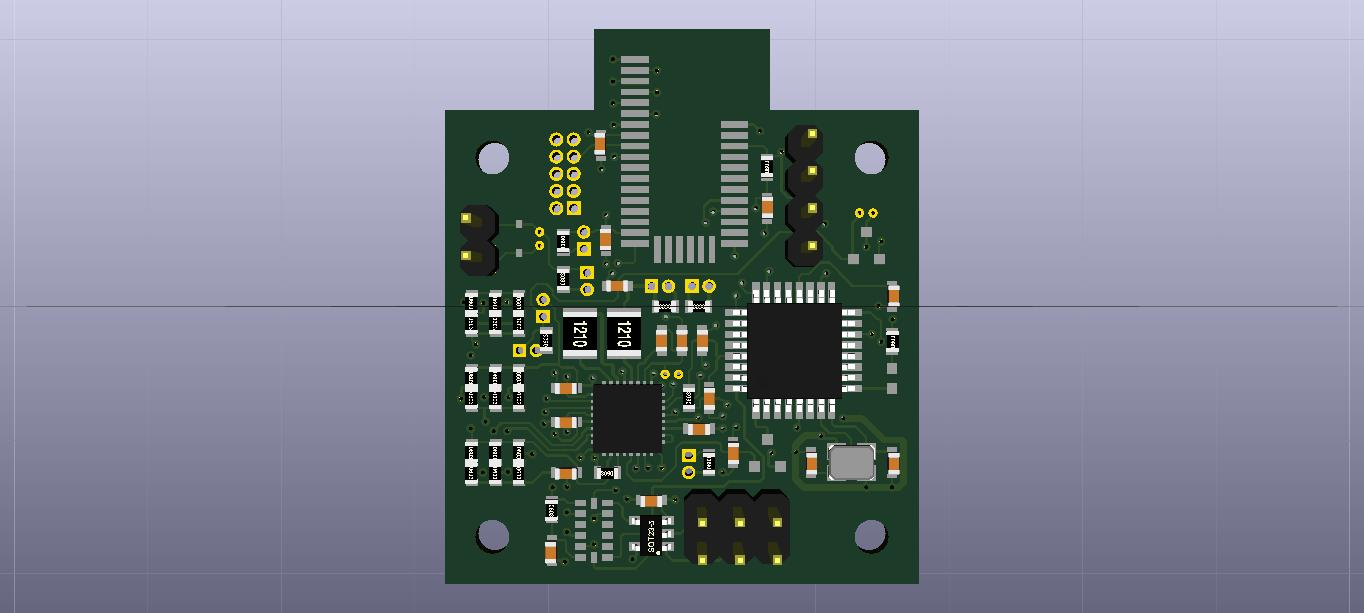
\includegraphics[height=6cm]{images/own_dwg/circuit/render.jpg}
  \end{center}
  \caption{\label{fig:pcb_render} Render of the final PCB}
\end{figure}

The borders between sections are most clearly visible in the power planes of design shown in Figure \ref{fig:pcb_planes}. Power planes for each subcircuit have been separated for testing the current consumption, and therefore the outlines of power planes follow the outlines of subcircuits.

\begin{figure}[htb]
  \begin{center}
    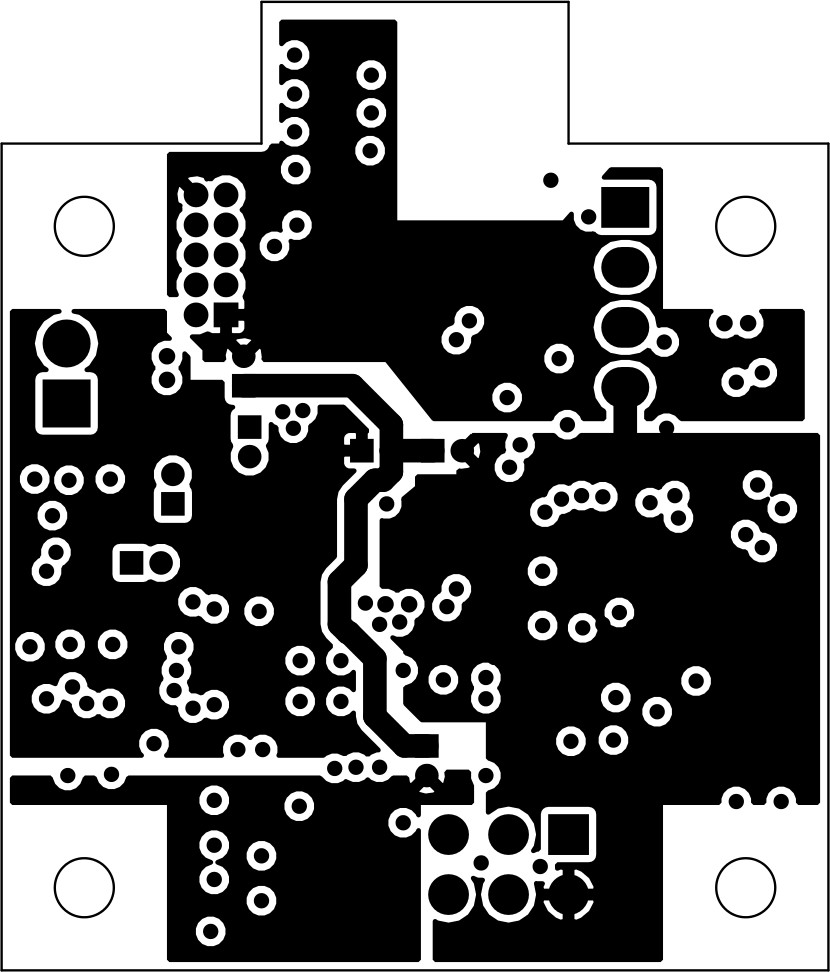
\includegraphics[height=6cm]{images/own_dwg/circuit/powerplane.jpg}
  \end{center}
  \caption{\label{fig:pcb_planes} Power planes of the PCB}
\end{figure}

In addition to mechanical and electrical properties, the PCB also acts as heat sink for mid-power components. In this circuit only LTC3331 needs special attention to thermal design, it is cooled by several vias under the pad of circuit into ground plane. As copper is an excellent conductor for heat, any thermal output from LTC3331 gets coupled to ground plane where it can spread to a wider area.

Battery holder is the only large component in design where G-forces might cause a problem. The holder is on the backside of the pcb, where it can be mounted using adhesives or it can be supported by the harvester top.

\subsection{Mechanical design of the harvester}
This section details the mechanical considerations for both piezolectric and electromagnetic harvesters. First material options are explored, then the design for generators is presented.

Material for the generator has a few requirements. It has to have at least as good temperature characteristics as the magnet being used and it must be hard enough to not deform under impacts. Low friction coefficient is desirable as this leads to smaller  frictional losses, and long time durability under wear is of course desired. Being lightweight and easily machinable are also desired characteristics. As the generator is small, volumetric cost of the material is of little concern. For the electro-magnetic generator design material ferromagnetism has to be considered. Table \ref{parameters_of_materials} displays comparison of different materials considered for this application.

\begin{table}[htb]
%% Taulukon teksti
\caption{\label{parameters_of_materials} Materials for the shaft of generator \cite{PlasticsInternational2015}, \cite{Etra}, \cite{Goodfellow} \cite{McCarr}.}
\begin{center}
\fbox{
\begin{tabular}{l l l l l l}
\textbf{Material}& 
\textbf{Hardness}& 
\textbf{Friction} & 
\textbf{Durability} & 
\textbf{Temperature}\\ \hline
PTFE(Teflon)      & Very low   & Lowest                      & Lowest    & -190... + 250 \degree C \\ 
Polycarbonate     & Very high  & High       & -         & -60... + 125 \degree C \\ 
PA 6 (Nylon)      & Low        & Medium                      & High      & -40... + 80 \degree C  \\ 
Oil-infused Nylon & Low        & Very low                    & Very high & -20... + 105 \degree C \\ 
Acryllic          & High       & -                           & -         & -40... + 70 \degree C \\ 
Polyacetal (POM C)& Medium     & Low                         & Low       & -50... + 105 \degree C \\ 
Carbon fiber     & Highest     & Highest                         & High       & ... + 80 \degree C \\ 
\end{tabular}
}

\end{center}
\end{table}

From the table \ref{parameters_of_materials} can be seen that there is no single best material for the harvester. Polycarbonate and carbon fibre  have excellent mechanical strength but they have high friction. Teflon and nylon have lower friction, but they have poor mechanical rigidity. 

In the end acryllic was chosen as the material of the harvester. While acryllic is not a best material by any single metric, it has the necessary properties. Acryllic is easy to machine and readily available which were decisive factors for the selection of acrylic over other materials. 

As the minimum diameter of the harvester is defined by piezoelement diameter of 34 mm, both generators are designed with 35 mm square bases. Both generators also use same mounting hole pattern for electronics - 2.75 mm holes at the corners of the square.

The generator was machined using slices of laser cut acrylic and standard acrylic tubing. The process is somewhat similar to 3D-printing, as several thin layers form up the final part. The acrylic parts used in generator are shown in figure \ref{fig:lasercut}.

\begin{figure}[htb]
  \begin{center}
    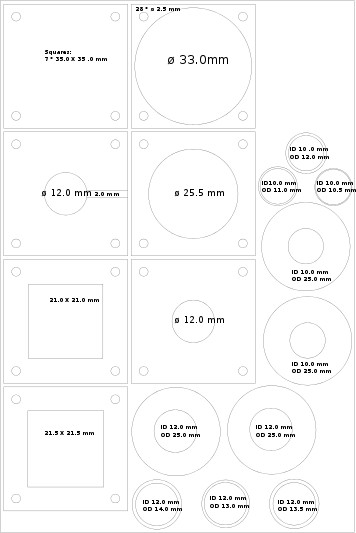
\includegraphics[height=15cm]{images/own_dwg/mechanical/layers.jpg}
  \end{center}
  \caption{\label{fig:lasercut} 150 * 150 mm sheet for laser cutting.}
\end{figure}

While the initial approach for building the shaft of the generator was to use lasercut rings to form the shaft, the process of lasercutting warped thinner rings and mechanical alignment of the rings was difficult. Therefore a standard 10 mm inner diameter 12 mm outer diameter tube was selected as the shaft.



%\section{Results} Practical
\clearpage
\section{Results and discussion}\label{sect:results}
\subsection{Test setup} \label{sect:lg_test_setup}
This section details the test setup on a vibration exciter. The harvesters were connected to vibration exciter Brüel \& Kjær type 4905 for measuring the frequency response and output power obtainable from the harvesters. Figure \ref{fig:emh_shaker} shows the test setup with electromagnetic harvester. Syscomp CircuitGear CGR201 oscilloscope was used to generate a test signal and take the measurements from the harvesters. Signal from function generator was amplified by Brüel \& Kjær power amplifier type 2707.

\begin{figure}[htb]
\begin{center}
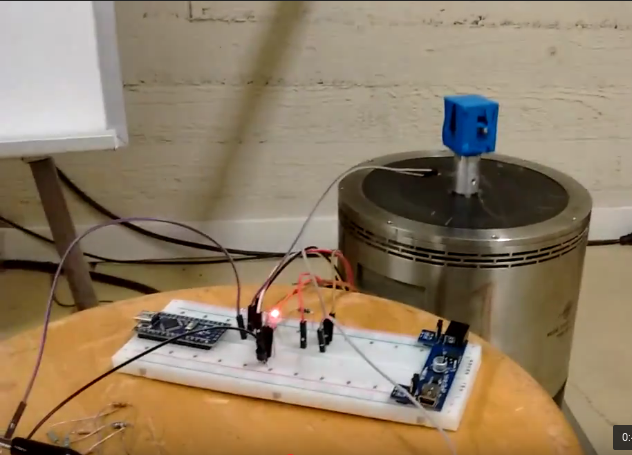
\includegraphics[height=8cm]{images/own_pic/shaker_setup/emh_shaker.png}
\end{center}
\caption{\label{fig:emh_shaker} Test setup for harvester.}
\end{figure}

The vibration exciter is electromagnetically driven platform which translates electrical signal into mechanical movement. Device under test is fastened onto test "head" of vibration exciter, and the acceleration seen by device is then controlled by electrical signal.

The test setup did not have feedback for the position of the harvester, so exact displacement or acceleration of the harvester is unknown. The output signal from the function generator had amplitude of 6 V peak-to-peak and the gain of power amplifier was set to 9.5 in testing.

\subsection{Experimental results of the electromagnetic harvester}
This section presents the experimental results from electromagnetic harvester on vibration exciter. The electromagnetic harvester was tested both on resistive load and while supplying power to a harvester board. 

The harvester was built according to design presented in Section \ref{sect:emh_design}. Figure \ref{fig:emh_final} shows the completed assembly. The rotor magnet can be seen suspended in the middle of assembly, the coil is formed on the upper half of the generator. A magnetic spring is formed by magnets on top and bottom sides of the harvester. 

\begin{figure}[htb]
\begin{center}
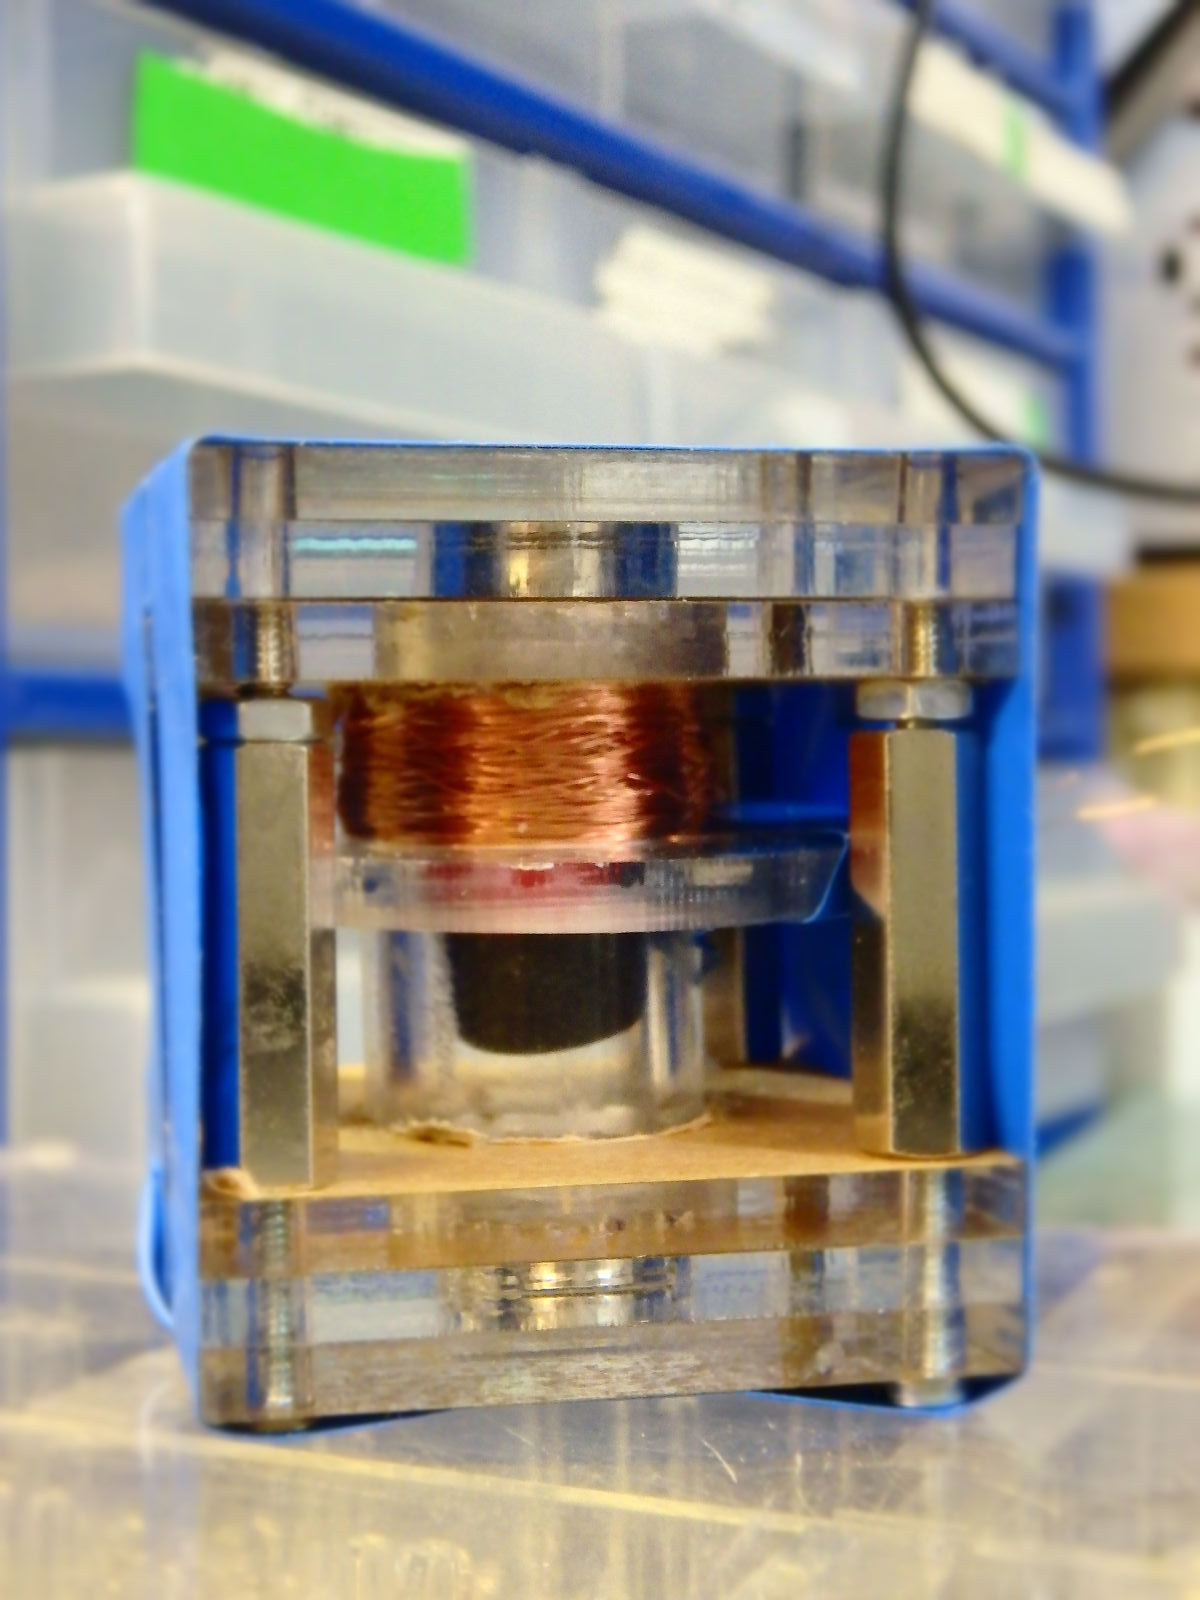
\includegraphics[height=8cm]{images/own_pic/inductive_harvester.jpg}
\end{center}
\caption{\label{fig:emh_final} Final prototype of electromagnetic harvester.}
\end{figure}

\subsubsection{Frequency domain results} \label{sect:emh_fd}
One of the original design goals of the harvester was to provide a wide-band energy harvester solution. This section presents the frequency domain response of the electromagnetic harvester.

Frequency domain response was obtained by sweeping a wide-band sine signal to power amplifier and measuring the open loop response from the harvester. The rotor magnet was stuck in the shaft of harvester at low frequencies, and the power output fell quickly on high frequencies. To solve this problem with friction, ferrofluid was applied to the rotor magnet. Ferrofluid is oil which has magnetic particles suspended in emulsion, these magnetic particles create effectively magnetic oil which stays on contact with the magnet surfaces. This approach has been used before in a ocean wave energy harvester \cite{Cheung2009}.

 After the application of ferrofluid electromagnetic harvester shows a strong resonance peak near 80 Hz as shown in Figure \ref{fig:inductive_fd_dry}. Above graph is the output in decibels, below is the phase shift of the response. Phase shift behaviour was not affected by ferrofluid lubrication. Usually the systems which have second order dynamics - such as the mass damper spring system - exhibit resonance peaks when the damping factor is low. It is can therefore be concluded that application of ferrofluid has resulted in lesser frictional losses. Amplitude response is also at higher level across all frequencies, suggesting a better overall performance of the harvester. 

\begin{figure}[htb]
\begin{center}
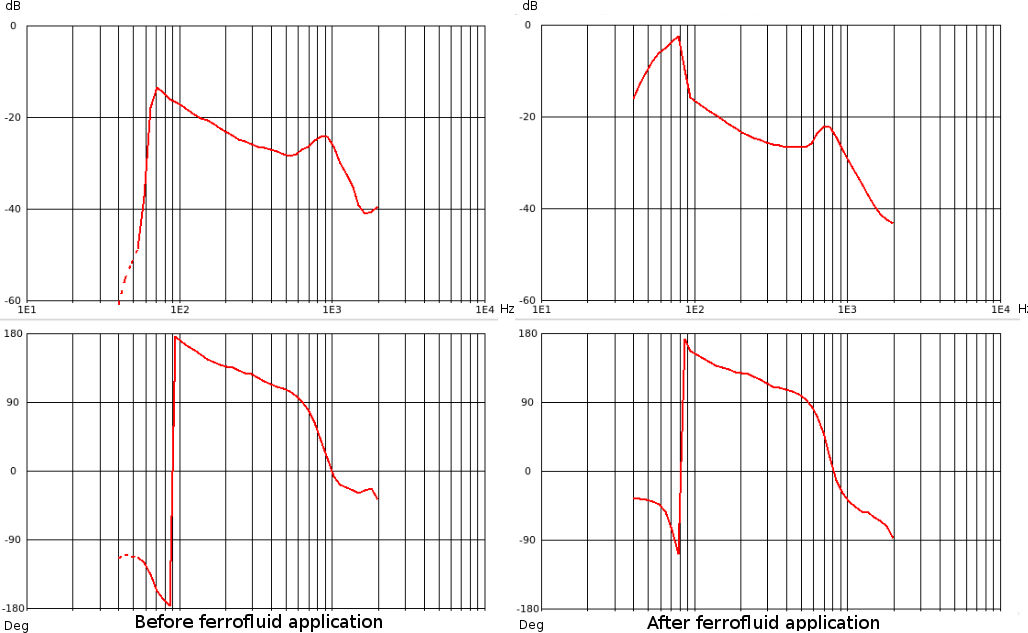
\includegraphics[width=\columnwidth]{images/own_measurement/generator_shaker/inductive_fd_combined.png}
\end{center}
\caption{\label{fig:inductive_fd_dry} Frequency domain response of electromagnetic harvester before and after application of ferrofluid. Above graph is the amplitude response, bottom is the phase shift. After application of ferrofluid the resonance peak is notably sharper, indicating a higher quality factor.  }
\end{figure}

The phase shift is almost exactly 180\degree \ at the resonance, which is somewhat curious result as the time domain results and theory predicted the voltage would peak at 90\degree \ phase when the acceleration is at zero and speed is highest. Amplitude does not have any specific meaning outside the context of this measurement and comparing output at different frequencies.  There is another resonance peak near 900 Hz, but this frequency is far above frequencies of interest for the application. The -3 dB bandwidth is $ \approx $ 10 Hz wide, which can be compared to results of Singh et al. \cite{Singh2012} referred in Section \ref{sect:background}. Singh et al. achieved approximately 5 Hz wide -3 dB bandwidth with piezoelectric harvester 70 Hz.


\subsubsection{Time domain results}\label{sect:lg_td}
The time domain waveforms of the electromagnetic harvester were measured on various loads and frequencies. After the open loop results were obtained, the tests were run again with different resistive loads to measure the power output. Finally the power output to the rectifier of the harvesting circuit of was measured. This section presents the test results. 

The magnet inside the harvester had a notable amount of friction which had to be overcome before any output could be obtained from the harvester. It was not possible to obtain very small signals from harvester, as any input strong enough to move the magnet resulted in a volt-scale output. Figure \ref{fig:inductive_65_open_dry} shows an example of waveforms obtained from harvester. 

\begin{figure}[htb]
\begin{center}
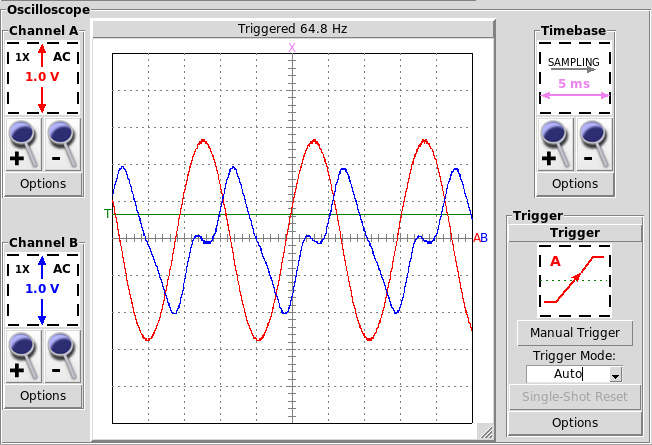
\includegraphics[height=10cm]{images/own_measurement/generator_shaker/inductive_td_open_65hz_dry.png}
\end{center}
\caption{\label{fig:inductive_65_open_dry} Open circuit response of the electromagnetic harvester. Red is the excitation waveform, blue is the open-circuit voltage from the harvester.}
\end{figure}

The waveforms presented in Figure \ref{fig:inductive_65_open_dry} have some curious features: the response from the harvester is asymmetric, there is a notable valley of no output on the rising edge of the signal while no such edge is visible on falling edge. It should be noted that these valleys do not necessarily correspond to the direction of gravity: the phase of input/output signal can be inversed at any point in the signal chain as the polarity of magnet, direction of the winding of coils, and connection of wires can change.

There seems to be a 90\degree \ phase shift between excitation and response. This phase shift was expected, as the excitation signal drives acceleration to exciter, so speed of the magnet reaches maximum at the zero-crossings of excitation. This observation matches well theory presented in Section \ref{sect:em_harvest}: Voltage is proportional to the rate of change of magnetic field. 

Amplitude of output is 2 V and the resistance of the coil was measured to be 34 $\Omega$ at DC. Inductive component of the coil impedance is negligible at the frequencies of interest, so only the resistive component needs to be considered. The Optimal load would then be 34 $\Omega$. When these values are substituted in time domain into Equation \ref{eq:generator_load_power} in Section \ref{sect:em_harvest} we obtain:

\begin{equation}\label{eq:emh_resistive_power_output}
  P_{load}(t) = V(t) \cdot \frac{ 34 \Omega }{ 34 \Omega + 34 \Omega } \cdot \frac{ V(t) }{ 34 \Omega + 34 \Omega } = \frac{V(t)^2}{136 \Omega}
\end{equation}

When peak amplitude of 2 V is inserted to the Equation \eqref{eq:emh_resistive_power_output} peak power is $ \approx 30 mW $. Root mean square (RMS) voltages are used to express the average power over time. RMS cannot be accurately calculated from given values, as the waveform is not  mathematically perfect. If the waveform is approximated as triangle wave, the RMS power would be 

\begin{equation} \label{eq:rms_power}
  P_{rms} = k \cdot P_{peak} = \frac{1}{\sqrt{3}} \cdot 30 mW \approx 17 mW 
\end{equation}
where $k$ is a constant multiplier for RMS power for triangle waves. 
If the excitation power was increased until rotor magnet audibly contacted the endstop magnets, there was no significant change in output voltage. One possible explanation is the valley in output waveform: maybe the rotor magnet was driven to near-contact to stator magnet and when the acceleration was reduced the rotor magnet was accelerated mainly by the magnetic interaction. The end result would be that the length of the valley in the output waveform would vary while the output amplitude would be limited by the magnetic interaction. While further exploration of this phenomenon would be interesting, the testing would be potentially destructive and therefore those experiments were left to future work.

This harvester cannot be used with the circuit designed in Section \ref{sect:electronic_design} as the output amplitude is only 2 V at any reasonable acceleration and frequency. The circuit would require minimum of 4 V to get out of the undervoltage lockout, and this is not achievable even by connecting the bridge rectifier as a voltage doubler because the energy harvesting input still has two diode drops which would keep the voltage below the required threshold.

Next test was done by connecting the harvester to a boost circuit based on TI BQ25504 \cite{bq25504}. BQ25504 has a boost-mode SMPS in energy harvesting input which is able to utilise input voltages as low as 80 mV after startup and it can start up at roughly 330 mV. The detailed description of the circuit is given in Section \ref{sect:BQ25504_schematic}. The issue with diode voltage drops was remedied by using schottcky-diodes connected as voltage doubler.

To measure the actual power output, a current-to-voltage converter $\mu$Current \cite{Jones2010} was connected in series to the output of harvester. Measurement was done at scale 1 V = 1 mA. Waveforms are shown in figure \ref{fig:inductive_vi_65}. It should be noted that the current channel might be saturated, as the $\mu$Current cannot produce output higher than 1.25 V.

\begin{figure}[htb]
\begin{center}
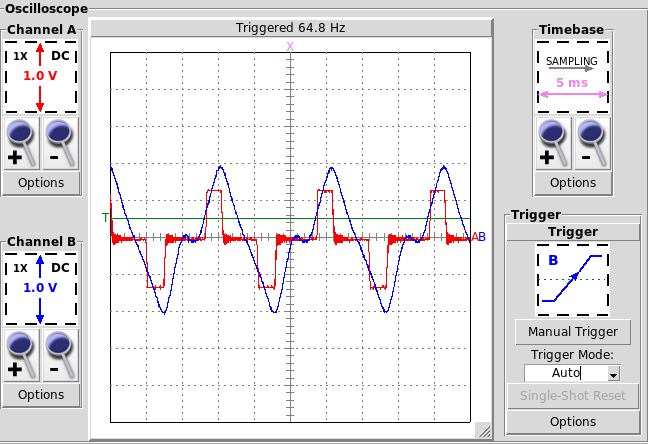
\includegraphics[height=10cm]{images/own_measurement/generator_shaker/inductive_td_harvesting_vi_65hz_ferro.png}
\end{center}
\caption{\label{fig:inductive_vi_65} Voltage and current waveform from harvester. Red is current, 1 V equals 1 mA. Blue is voltage from the terminals of harvester before rectification.}
\end{figure}

The waveforms are as expected, there is no current flowing while the voltage is low. When the voltage rises to roughly one volt, current starts to flow charging the output capacitor. When the input voltage starts to decrease, no more current flows to the capacitor. Accuracy of amplitude of current measurement is questionable because of potential saturation of the measuring instrument.

It is worth noting that the voltage rises to open-loop maximum amplitude of 2 V as the loading on the harvester decreases as the voltage on capacitor increases. This indicates that maximum theoretical peak power output of $\approx$ 30 mW is not reached at any point. 

Power waveform of the harvester is presented in Figure \ref{fig:inductive_power_65}. The waveform is calculated by multiplying the voltage and current. Because the current is scaled at 1 mA = 1 V, the result can be read as 1 V = 1 mW. While absolute value of power is questionable because of the potentially saturated instrument, the waveform itself is correct.  

\begin{figure}[htb]
\begin{center}
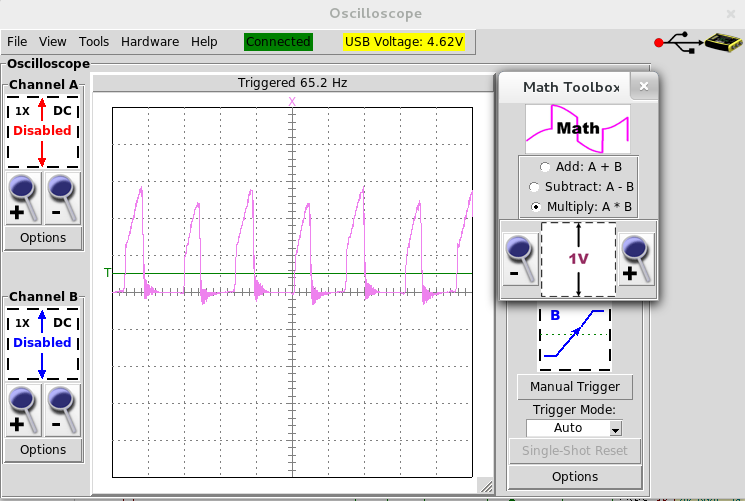
\includegraphics[height=10cm]{images/own_measurement/generator_shaker/inductive_td_harvesting_power_65Hz_ferro.png}
\end{center}
\caption{\label{fig:inductive_power_65} Power waveform from harvester. Pink is power, 1 V equals 1 mW.}
\end{figure}

Graphically read average power output is 0.375 mW. One possible reason for the greatly lower power output was the capacitors in voltage doubler structure: the voltage doubler has series capacitance of 10 $\mu$F, which has a reactive impedance of

\begin{equation}
  X_c = \frac{1}{2 \pi f C}  = \frac{1}{2 \pi \cdot 65 Hz \cdot 10\mu F} \approx 245 \Omega
\end{equation}
at 65 Hz. Total output impedance of circuit would be approximately 280 $\Omega$, which would limit the output current to approximately 7 mA. This theory was tested by simulating the equivalent model of input section of harvester circuit. Simulation model and results are shown in Figure \ref{fig:simulated_doubler}.

\begin{figure}[htb]
\begin{center}
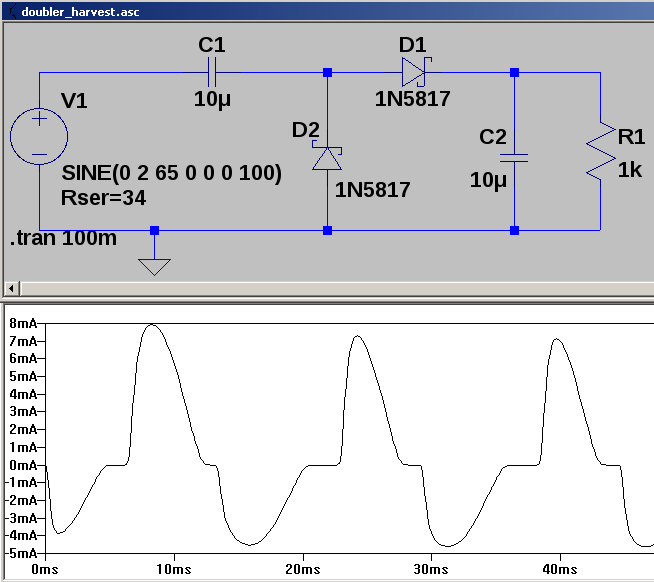
\includegraphics[height=10cm]{images/own_dwg/simulation/voltage_doubler.png}
\end{center}
\caption{\label{fig:simulated_doubler} LTSpice model of energy harvester input section.}
\end{figure}

The simulated data confirms the effect of input capacitor to current output of the system. Current is limited to roughly 7 mA. Simulated power output was on average 2.0 mW. If the measured current is assumed to be limited by saturation, and if we assume that simulated current of 8 mA peaks would be correct, the calculated power output from experimental result would be 

\begin{equation}
  P_{true} = P_{simulated} \cdot \frac{I_{simulated}}{I_{real}} = 0.375 mW \cdot \frac{7 mA}{1.25 mA} = 2.1 mW.
\end{equation}

After correcting the experimental current with the simulated value, a lot more reasonable value of approximately 2 mW of generated power is obtained. 

This section presented the time-domain results of the electromagnetic harvester on a vibration exciter test platform. Approximately 30 mW peak power was obtained, RMS power of 17 mW was achieved to resistive load and power output to harvester was determined to be in range between 0.4 mW and 2 mW. 

\subsection{Experimental results of the piezoelectric harvester}
\subsubsection{Frequency domain results} \label{sect:piezo_fd}
The frequency domain response of the piezoelectric harvester was obtained in similar manner as with the electromagnetic harvester detailed in Section \ref{sect:emh_fd}. The excitation signal was swept across a wide spectrum and output from the harvester was measured. Frequency domain results are presented in this section.

The frequency sweep result on open circuit is shown in Figure \ref{fig:piezo_fd}. A resonance peak can be found at 334 Hz. Similarly to the electromagnetic harvester, the slope is a lot steeper on the frequencies above the resonance peak than below. 

\begin{figure}[htb]
\begin{center}
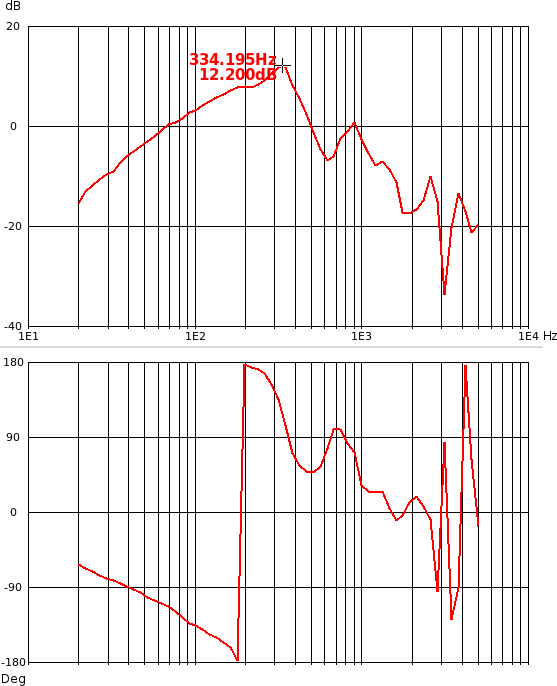
\includegraphics[height=10cm]{images/own_measurement/generator_shaker/piezo_fd_open_2_3.png}
\end{center}
\caption{\label{fig:piezo_fd} Frequency response of piezoelectric harvester}
\end{figure}


The peak frequency is somewhat poorly suited to the environment in the tyre presented in Section \ref{sect:tyre_environment}, as the peak response is significantly above peak frequencies encountered in the tyre. Usually the frequency is tuned downwards by adding mass to the harvester, however this approach is not feasible in this application as the proof mass is limited to avoid damage to the piezoelement due to excessive strain. As the peak frequency was identified near 330 Hz, the time domain analysis were performed on the harvester. Next section details the voltage, current and power outputs into varied loads.

\subsubsection{Time domain results}\label{sect:piezo_td}
This section presents the time-domain results of the piezoelectric harvester. The test setup of the piezoelectric harvester was similar to the test setup of the electromagnetic harvester, details of the test setup are given in Section \ref{sect:lg_test_setup}. Unlike the electromagnetic harvester, this piezoelectric harvester did not have any obvious minimum acceleration before the friction would be overcome and therefore even very small signal was obtainable. Likewise no maximum value for output signal was found by increasing the power to the vibration exciter. The function generator output signal was held at 6 volts peak-to-peak for the time domain tests and at 3 volts peak-to-peak for frequency domain tests to limit the loosening of the screws by vibration. Gain of the power amplifier was fixed at 9.5.

The piezoelectric harvester was characterised by high output voltages at high output impedance. Open loop response is shown in Figure \ref{fig:piezo_td_open}. The output was not a clean sine-resembling signal as with the electromagnetic harvester, it has sharp downwards peaks and a lot of high-frequency distortion.

\begin{figure}[htb]
\begin{center}
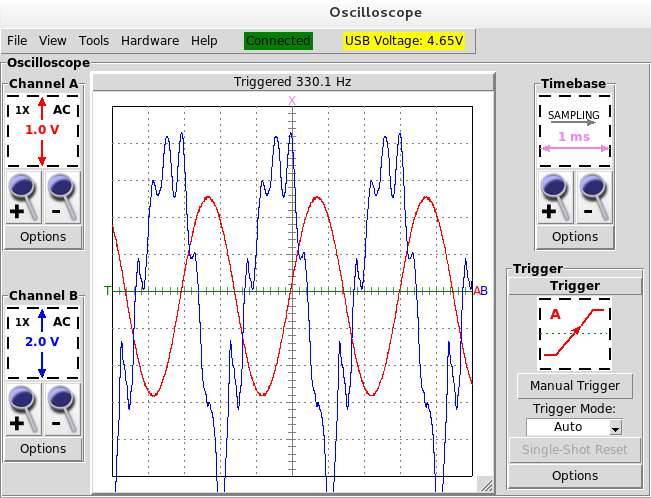
\includegraphics[height=10cm]{images/own_measurement/generator_shaker/piezo_td_open_330hz_2_2.png}
\end{center}
\caption{\label{fig:piezo_td_open} Open loop response from the piezoelectric harvester. Red is the excitation signal, blue is the response.}
\end{figure}

While output signal is off the scale, negative peaks were measured at -12 V. Peak-to-peak amplitude was therefore roughly 20 V. The search for the maximum power point was started by modeling the circuit as RC- high pass filter shown in Figure \ref{fig:rc_highpass} with piezo capacitance as the series capacitor and load as the resistor. 

\begin{figure}[htb]
\begin{center}
\includegraphics[height=4cm]{images/cited/hyperphysics.jpg}
\end{center}
\caption{\label{fig:rc_highpass} RC high pass filter \cite{hyperphysics}.}
\end{figure}

The frequency domain results presented in Section \ref{sect:piezo_fd} were used to find the maximum output frequency at 330 Hz. This frequency was taken as the target cut-off frequency for the RC-filter equation:

\begin{equation}
\begin{split}
  F_c &= \frac{1}{2 \pi R C} \\
  R   &= \frac{1}{2 \pi C F}  = \frac{1}{2 \pi \cdot 39 nF \cdot 330 Hz} \approx 12 400 \Omega 
\end{split}
\end{equation}

Theory would predict the maximum power point to be near the cut-off frequency, so the generator was tested with 18 k$\Omega$, 12 k$\Omega$ and 9 k$\Omega$ resistive loads. The peak voltages and calculated power into the load are presented in Table \ref{tbl:piezo_harvester_shaker_output}. The power is calculated by approximating the waveform as a clean sine calculating RMS power from peak voltage values. Method is similar to Equation \eqref{eq:rms_power} presented in Section \ref{sect:lg_td}, but the multiplier $k$ is $\sqrt{2}$ instead of $\sqrt{3}$ as the waveform is approximated as a sine rather than a triangle. While the absolute value of the power output has approximation error, the waveforms obtained with 18 k$\Omega$ and 12 k$\Omega$ are similar enough for comparing the outputs between the loads. On 9 k$\Omega$ load the waveform was clearly more distorted, and therefore calculation for power has greater approximation error.

\begin{table}[htb]
\caption{\label{tbl:piezo_harvester_shaker_output} Output power of piezo harvester at 18 k$\Omega$, 12 k$\Omega$ and 9 k$\Omega$ loads.}
\begin{center}
\fbox{
\begin{tabular}{r l l}
\textbf{Load}          & \textbf{Amplitude} 		& \textbf{Power\textsubscript{rms}}	\\ \hline
18 k$\Omega$  & 7 volts	& 1.36 mW \\ 
12 k$\Omega$  & 6 volts	& 1.50 mW \\ 
9 k$\Omega$  & 4 volts 	& 0.89 mW
\end{tabular}
}
\end{center}
\end{table}

The waveforms from 12 k$\Omega$ load and 9 k$\Omega$ load are shown in Figures \ref{fig:piezo_td_12k} and \ref{fig:piezo_td_9k} for comparing the amount of distortion. While both waveforms show a clear high-frequency content, possibly caused by resonant frequency of piezo element itself, the heavier loading causes a significant distortion on the waveform.

\begin{figure}[htb]
\begin{center}
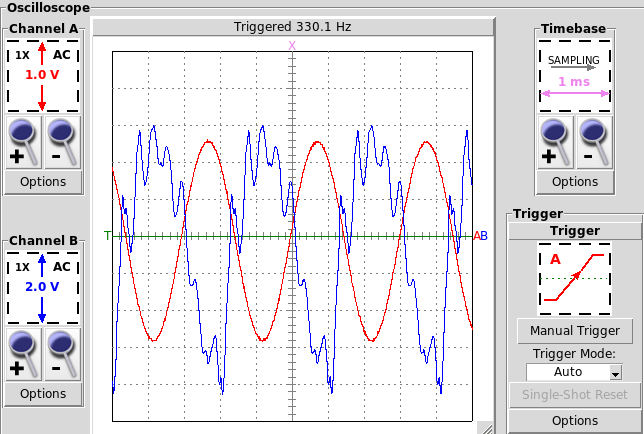
\includegraphics[height=10cm]{images/own_measurement/generator_shaker/piezo_td_12k_330hz_2_2.png}
\end{center}
\caption{\label{fig:piezo_td_12k} Piezoelectric harvester under 12 k$\Omega$ load. Red is the excitation signal, blue is the response.}
\end{figure}

\begin{figure}[htb]
\begin{center}
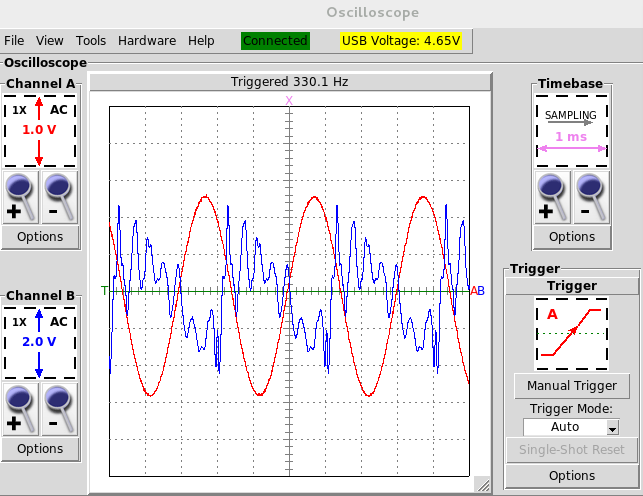
\includegraphics[height=10cm]{images/own_measurement/generator_shaker/piezo_td_9k_330hz_2_2.png}
\end{center}
\caption{\label{fig:piezo_td_9k} Piezoelectric harvester under 9 k$\Omega$ load. Red is excitation signal, blue is response.}
\end{figure}

The waveform on Figure \ref{fig:piezo_td_9k} resembles almost a saw-tooth wave. Regardless of actual RMS value, it can be confidently said that the power output is smaller under 9 k$\Omega$ load than under 12 k$\Omega$ load. Therefore maximum power point can be concluded to be near 12 k$\Omega$ load at 330 Hz. 

After testing the behaviour of piezoelectric harvester on resistive loads, power output to the harvester through rectification was tested. While the electromagnetic harvester had a notably higher output to resistive load, rectification drops voltage and therefore high-voltage characteristic of piezoelectric harvester is advantageous for rectification. 

As with the electromagnetic harvester, current was measured using $\mu$Current at 1 mV / $\mu$A setting. While the electromagnetic harvester suffered from reactance of series capacitance limiting the output of the harvester, output impedance of piezoelectric harvester is a lot higher than impedance of additional series capacitor and therefore the output was not impaired by the coupling capacitance. The VI-waveforms are shown in Figure \ref{fig:piezo_td_vi}. 

\begin{figure}[htb]
\begin{center}
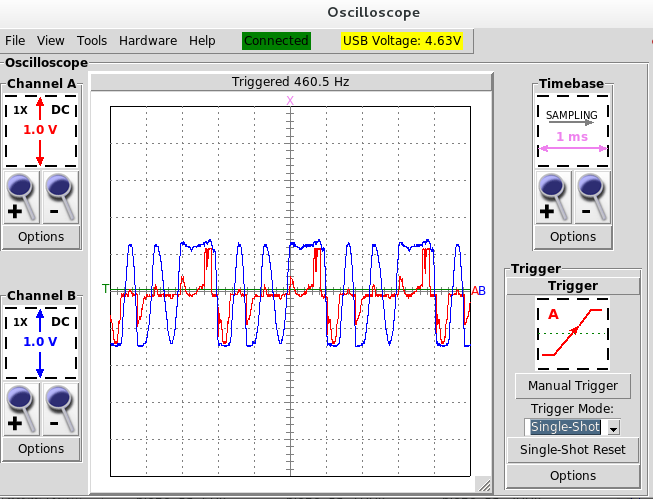
\includegraphics[height=10cm]{images/own_measurement/generator_shaker/piezo_td_vi_330hz_2_3.png}
\end{center}
\caption{\label{fig:piezo_td_vi} VI-waveforms of piezoelectric harvester into rectifier. Blue is voltage, red is current with scaling of 1 mA / V. Current does not follow the voltage and voltage is clamped by diodes.}
\end{figure}

Output of the piezoelectric harvester does not follow the excitation in a similar manner to the electromagnetic harvester. The output voltage is clamped by the diodes of rectification circuit, and the current waveform does not follow the voltage waveform. Power output waveforms have been presented in Figure \ref{fig:piezo_td_power}. As before, the output can be read as 1 V = 1 mW. 

\begin{figure}[htb]
\begin{center}
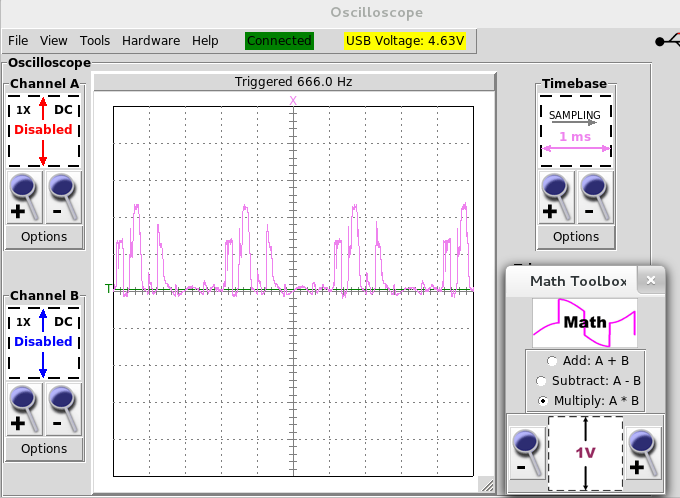
\includegraphics[height=10cm]{images/own_measurement/generator_shaker/piezo_td_power_330hz_2_3.png}
\end{center}
\caption{\label{fig:piezo_td_power} Power waveform of piezoelectric harvester. Scaling is 1 mW / V.}
\end{figure}

While excitation frequency of 330 Hz was not clearly visible in VI-waveforms, the rectified signal is clearly double of 330 Hz. Graphic integration suggests the power output to be in order of hundreds of microwatts, with peak power output being approximately 2.4 mW. 

It can be concluded that piezoelectric harvester produces most of the power at the excitation frequency, any output from the internal resonances are negligible in comparison to energy obtained from the external actuation.

\subsection{Harvesting circuit results}
\subsubsection{Revisited circuit design}\label{sect:BQ25504_schematic}
While the original idea was to use the circuit presented in Section \ref{sect:electronic_design} for testing the system-level performance, it became obvious that the harvesters cannot produce output levels required by the circuit. A new simplified harvesting circuit was designed to test the performance of the harvester inside the tyre. The harvester design is presented in this section.

According to Rouvala, M. \cite{Rouvala2015} best way to utilise low output levels is to chain voltage multiplier circuit stages to produce higher DC-level and then use a boost circuit to bring the harvested output into desired level. A few ICs from different manufacturers were considered for the new circuit, namely Seiko S-882z \cite{SeikoInstruments2010} charge pumps, Linear Technology LTC3105 \cite{ltc3015} boost charger and Texas Instruments BQ255xx -series boost chargers. As Seiko ICs are not readily available and LTC3105 requires high start-up currents, BQ25504 \cite{bq25504} was chosen as the core for the harvesting circuit. The schematic of harvesting circuit is presented in Figure \ref{fig:bq25504} and Figure \ref{fig:bq25504_mounted} shows the assembled circuit mounted on top of the piezoelectric harvester.


\begin{figure}[htb]
    \centering
    \def\svgwidth{\columnwidth}
    \input{images/own_dwg/circuit/bq25504.pdf_tex}
    \caption{\label{fig:bq25504} Schematic of the revised harvester circuit. Inputs are to left, both AC and DC input is supported. Resistors R1 and R2 set the maximum power point tracking point. Resistors R3 ... R9 set operation points: such as target voltage as 3.3 V, power good thresholds and undervoltage lockout threshold at 2.2 V. C5 is the supercapacitor for storing energy, C7 is a ceramic capacitor for rejecting high-frequency noise. C3 provides high-frequency filtering for switched power supply noise and C4 is bulk capacitance for load. Over Temperature shutdown treshold (OT\_PROG) is set to 120 $\degree$C by pulling OT\_PROG to a high voltage level. VBAT\_OK signal is a digital output which can be used to wake sensor platform when enough energy has been stored for taking a measurement and transmitting data.}
\end{figure}

\begin{figure}[htb]
\begin{center}
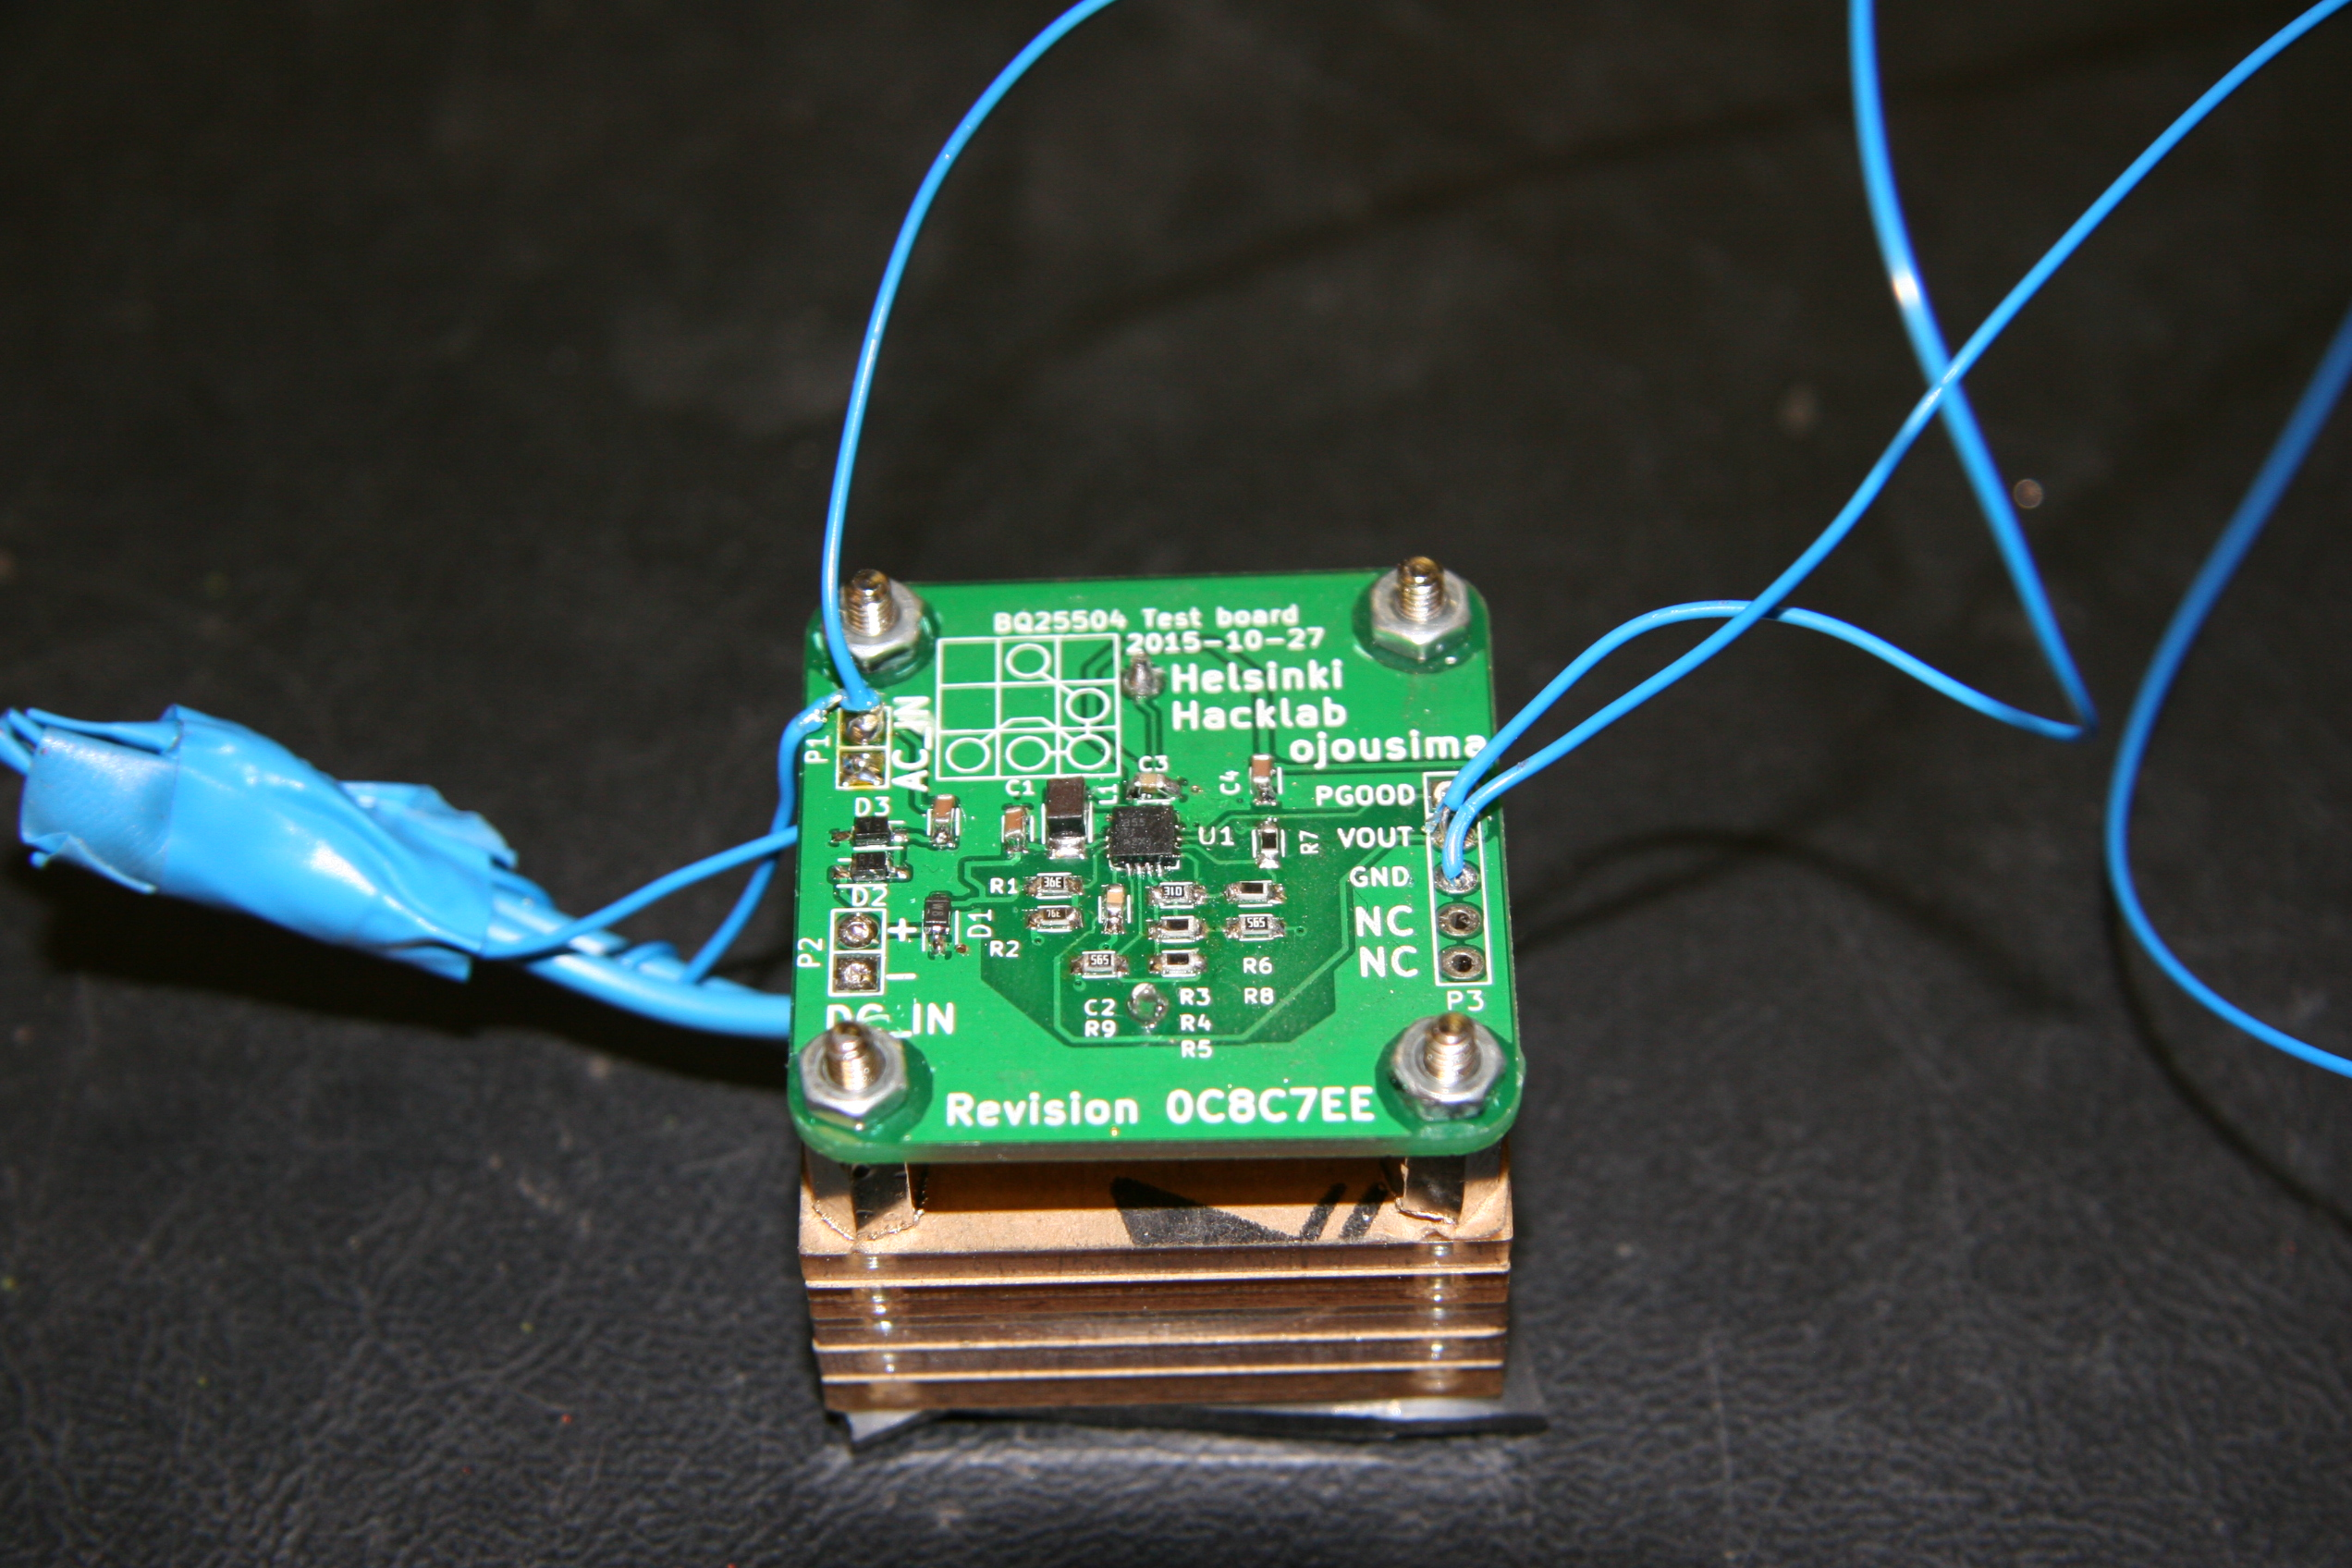
\includegraphics[height=8cm]{images/own_pic/tyre_fixture/piezo_bq_desk.jpg}
\end{center}
\caption{\label{fig:bq25504_mounted} BQ25504-based harvesting circuit mounted on piezoelectric harvester.}
\end{figure}

The revised harvesting circuit is able to start at 0.33 V input DC voltage, or at near 0.4 V RMS amplitude AC voltage contrasted to 5 V DC level of LTC3331-based circuit. A supercapacitor was chosen as energy storage for easy measurement of accumulated harvested energy. The supercapacitor was model EECRG0V155VN \cite{panasonic_scap} with 3.6 V maximum voltage and 1.5 F nominal capacitance. 

Maximum power point tracking is provided by sampling open-loop voltage of the circuit through voltage divider R1 and R2 every 16 seconds into capacitor C2. After the sample has been stored into the capacitor, BQ25504 attempts to set the current taken from the input so that V\textsubscript{IN} matches V\textsubscript{REF}. 

This form of MPPT is not adjustable by an external microcontroller: while digital potentiometers exist, their current consumption far exceeds the low-power requirements of the circuit. Therefore a fixed ratio had to be set for the circuit. The ratio was set to 80 \% to avoid overloading the piezoelement, as it was previously found in section \ref{sect:piezo_td} that overloading the element has a disastrous effect on efficiency of piezoelectric harvesting whereas underloading has much less pronounced effect on the efficiency.

Resistors R3 through R9 set various operation points for the circuit. Output voltage was set to 3.3 V, and power good -threshold was set to 3 V on charging and 2.2 V on discharging. 

The circuit was built and found to work with both harvester designs on the vibration exciter. As the circuit was usable, further work was carried out using this circuit. Next section details the measurement of the supercapacitor parameters after it was soldered in the circuit.

\subsubsection{Measuring the supercapacitor parameters}
As the energy storage used in the circuit is a supercapacitor and all subsequent measurements are based on values measured from the supercapacitor, the supercapacitor was characterised in-circuit to obtain more accurate values for the system performance. The measuring process and the results are presented in this section.

Application note AN1005 from Cap-XX \cite{an1005} details a simple process for measuring supercapacitor capacitance and Equivalent Series Resistance (ESR). The supercapacitor is first charged to a target voltage and then discharged through a resistor. The parameters are then read from the discharge waveform. A 100 ohm resistor was used as the discharging resistance, the discharge waveform is shown in Figure \ref{fig:scap_discharge}. 

\begin{figure}[htb]
\begin{center}
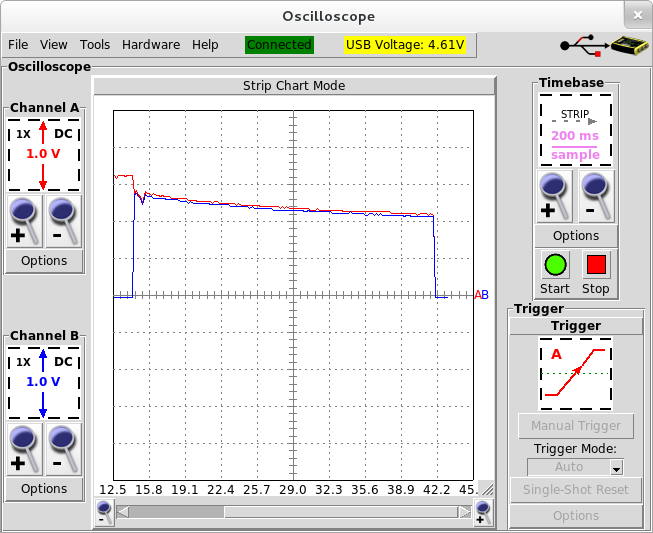
\includegraphics[height=8cm]{images/own_measurement/circuit/discharge.png}
\end{center}
\caption{\label{fig:scap_discharge} Discharge waveform. Red is the capacitor voltage, blue is voltage over 100 ohm resistor.}
\end{figure}

The initial discharge current can be calculated with voltage over resistor:

\begin{equation}
  I_{initial} = \frac{V_{initial}}{R} = \frac{2.75 V}{100 \Omega} \approx 27.5 mA 
\end{equation}

With the initial discharge current and voltage drop known, ESR can be calculated:

\begin{equation}
  ESR = \frac{V_{0} - V_{initial}}{I_{initial}} = \frac{3.25 V - 2.75 V}{27.5 mA} \approx 18.2 \Omega
\end{equation}

With ESR known, it is possible to calculate capacitance from the discharge time:

\begin{equation}
\begin{split}
  V_t                            &= V_{initial}e^{-t/R_{tot}C} \\
  \frac{V_t}{V_{initial}}                &= e^{-t/R_{tot}C} \\
  ln\left(\frac{V_t}{V_{initial}}\right) &= \frac{-t}{R_{tot}C} \\
  C                              &= \frac{-t}{R_{tot}} \frac{1}{ ln\left(\frac{V_t}{V_{initial}}\right)} = \frac{41.6-14.4}{100 + 18.2} \frac{1}{ ln\left(\frac{2.75 V}{3.25 V}\right)} \approx 1.38 F
\end{split}
\end{equation}

Therefore the capacitor ESR was found to be 18.2 $\Omega$ and capacitance 1.37 F. This is well within the published \cite{panasonic_scap} initial values of ESR < 30 $\Omega$ and capacitance of 1.5 F -20 \% ... + 80 \%, and therefore the results can be considered reliable. 

As the devices were proven in a laboratory setting, further test was carried out to determine the power output in a simulated drive inside a tyre. The test setup and results are detailed in next section.

\subsection{Performance inside tyre}
The final experiment was to install the piezoelectric harvester with revisited electronics inside the tyre and simulate driving conditions with a dynamometer platform. Piezoelectric harvester was chosen for the final tests as it was able to produce output even with small excitation unlike electromagnetic harvester which required a minimum impact before producing power. The test results are presented in this section. 

The harvester was glued to the inner lining of the tyre as shown in Figure \ref{fig:harvester_potted} and electrical connections were brought through a slip ring for instrumentation. The tyre was installed to rig presented in Figure \ref{fig:tyre_platform} and the tyre was driven at various speeds and loads. 

\begin{figure}[htb]
\begin{center}
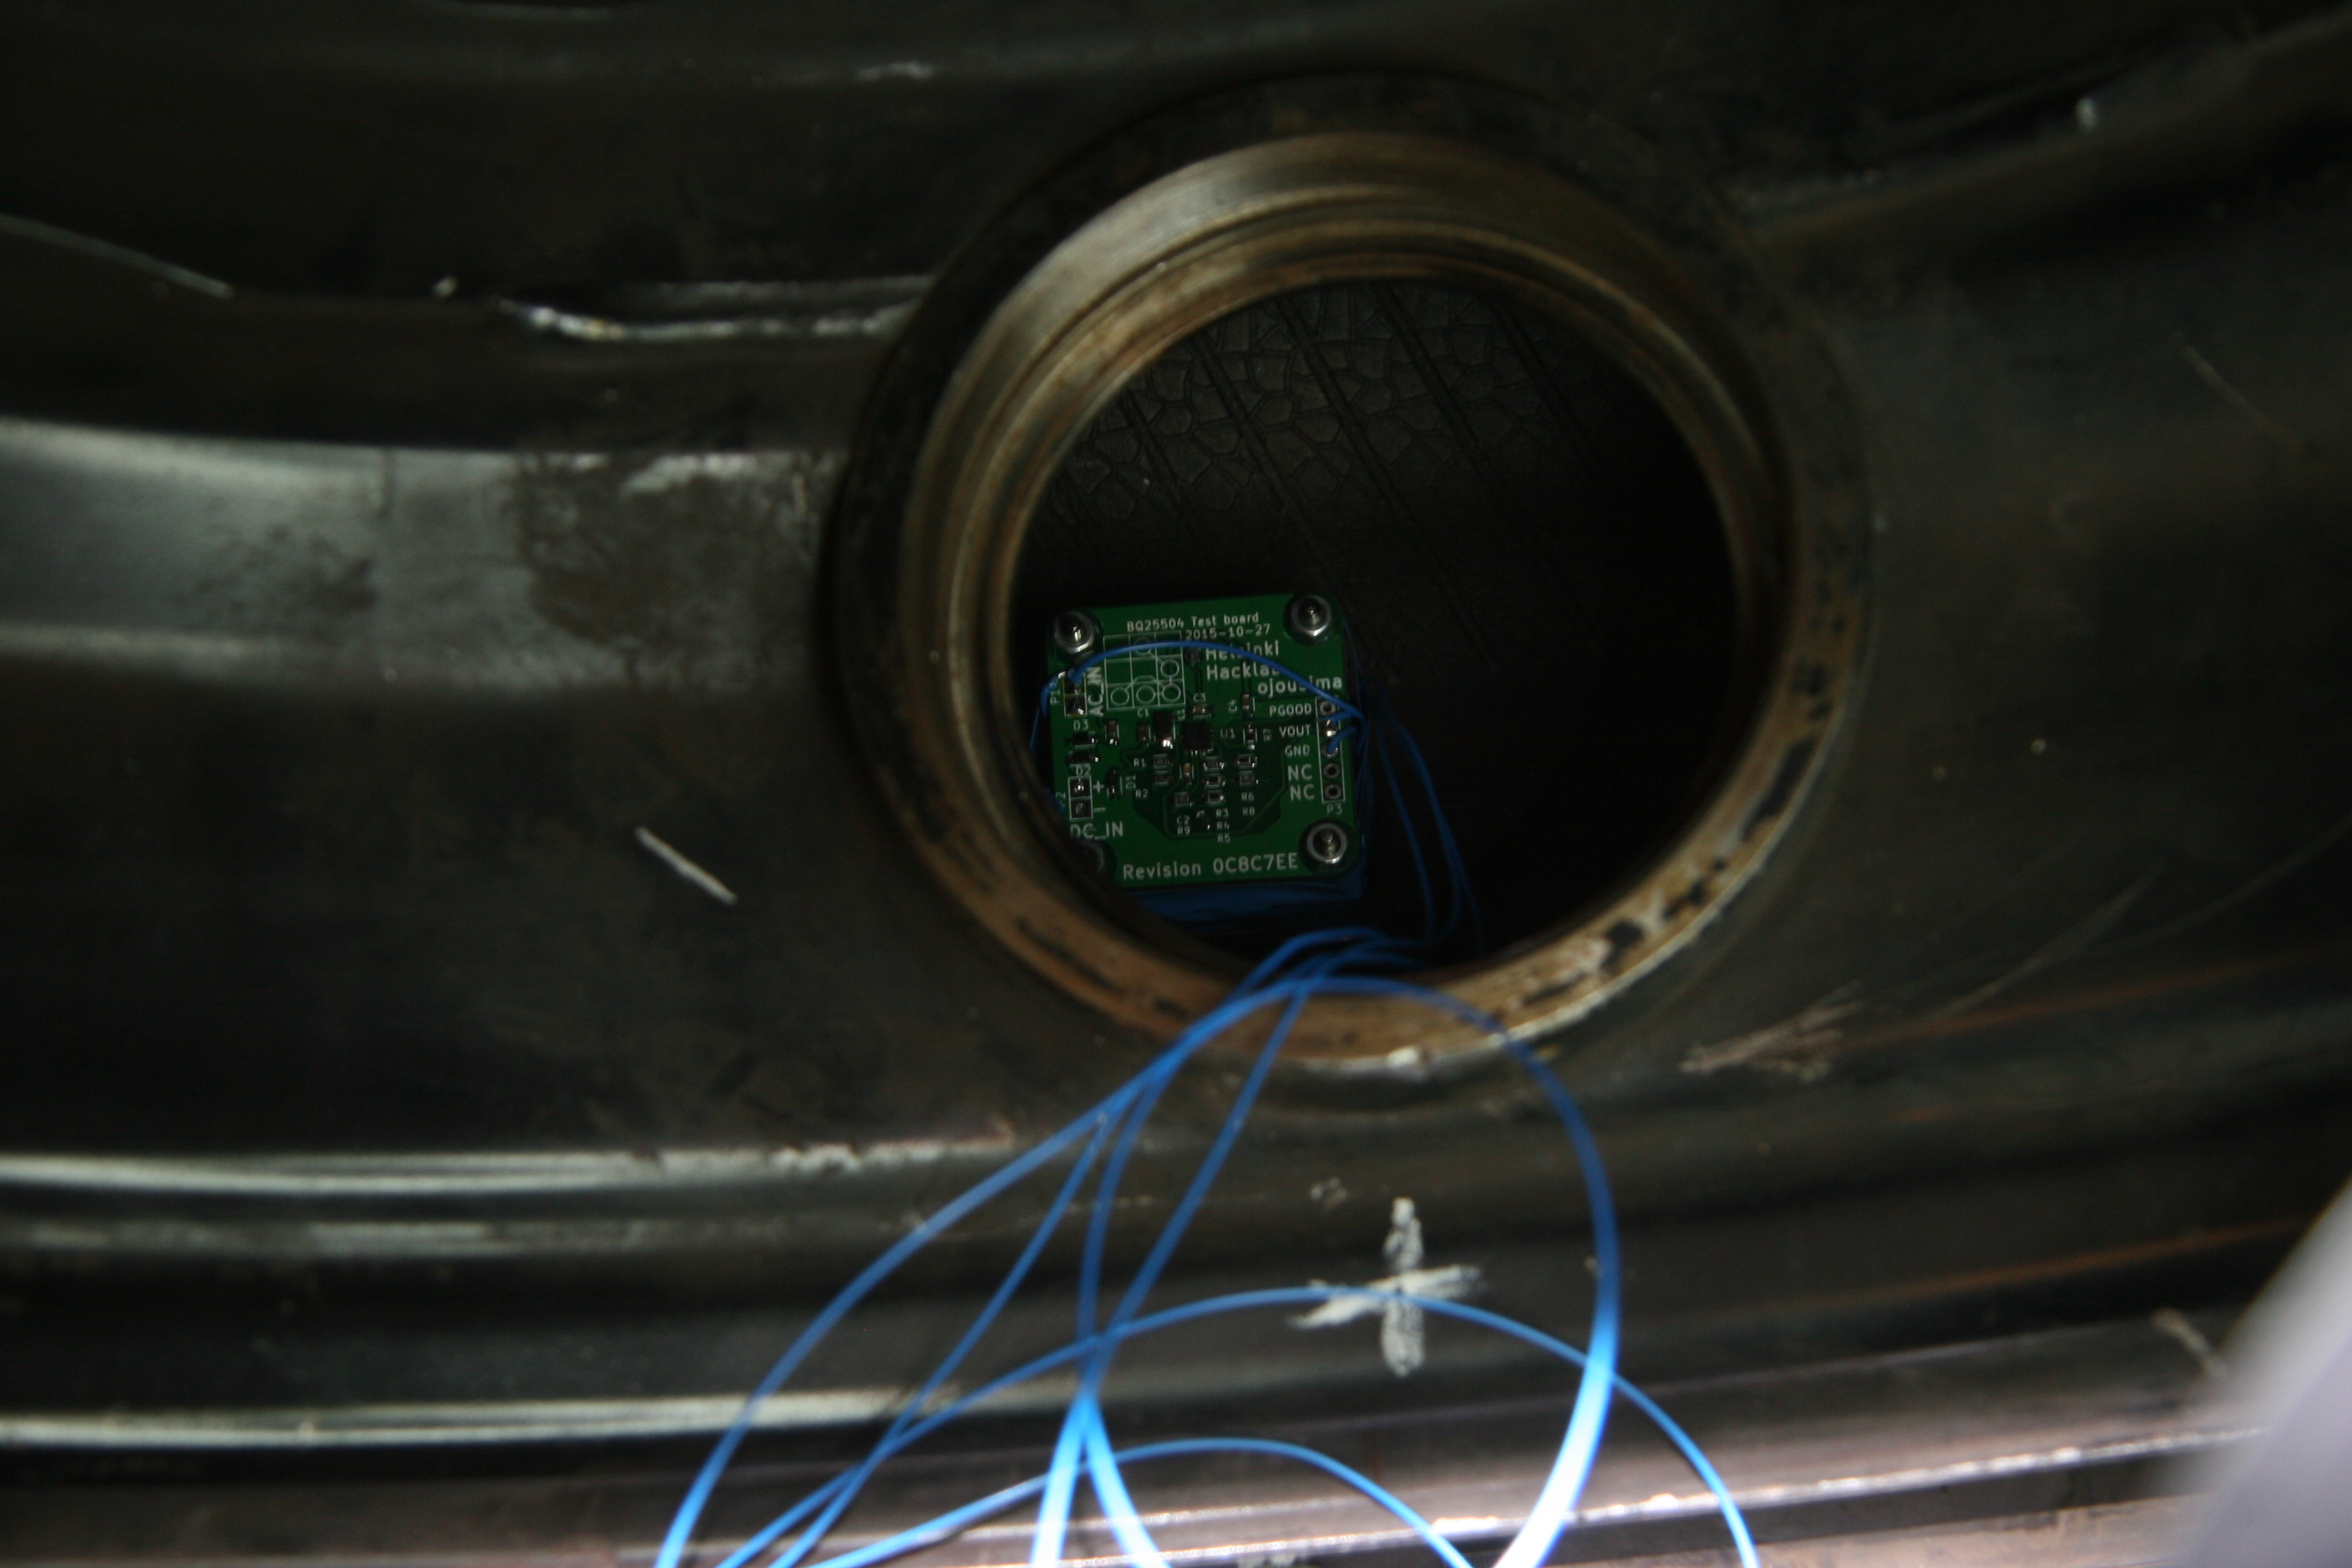
\includegraphics[height=8cm]{images/own_pic/tyre_fixture/piezo_bq_mount.jpg}
\end{center}
\caption{\label{fig:harvester_potted}Piezoelectric harvester mounted inside the tyre.}
\end{figure}

\begin{figure}[htb]
\begin{center}
\includegraphics[height=8cm]{images/own_pic/tyre_fixture/dyno.jpg}
\end{center}
\caption{\label{fig:tyre_platform} Tyre assembled in test platform.}
\end{figure}

The supercapacitor was fully charged before installing in tyre. Measurements were taken next day when the voltage had stabilised near 2.670 V. Tyre was driven at varied speeds and loads. Power output was estimated based stored voltage in supercapacitor before and after the test. The voltage was measured with NI 9215 \cite{ni9215} which has precision required for measuring millivolt-scale differences. 

\begin{table}[htb]
\caption{\label{tbl:piezo_harvester_tyre_output} Measured values from tyre test setup.}
\begin{center}
\fbox{
\begin{tabular}{l l l l l r}
\textbf{Speed} & \textbf{Load} 		& \textbf{V\textsubscript{0}} & \textbf{V\textsubscript{end}} & \textbf{Duration} & \textbf{Power}	  \\ \hline
20 km / h      & 1 kN 		        & 2.674 V        & 2.674 V          & 600 s             & $ 0 \mu W $      	\\ 
20 km / h      & 2 kN 		        & 2.674 V        & 2.676 V          & 600 s             & $ 13 \mu W $      	\\
30 km / h      & 1 kN 		        & 2.676 V        & 2.680 V          & $ \approx $ 300 s     & $ \approx 50 \mu W $       	
\end{tabular}
}
\end{center}
\end{table}

Regrettably the supercapacitor leads to PCB broke down during measurement at 30 km / h and therefore no accurate data was obtained at that speed. However, the results suggest that average power of 50 $\mu$W was obtained from the harvester at 30 km / h speed. The harvesting circuit has a considerable leakage of power at initial charging. This is probably because of the leakage characteristics of the supercapacitor shown in Figure \ref{fig:scap_leakage}. Initial leakage current of a supercapacitor can be in order of tens of microamperes, and it will decrease over course of several days to a specified value \cite{Mars2012}.

\begin{figure}[htb]
\begin{center}
\includegraphics[height=8cm]{images/cited/mars2012.png}
\end{center}
\caption{\label{fig:scap_leakage} Supercapacitors have high initial leakage \cite{Mars2012}.}
\end{figure}

This section presented the real-world power output of piezoelectric harvester. Usable, rectified and regulated power output was at least 13 $\mu W$. Further experiments suggest the energy output is near 50 $\mu W$ at 30 km / h under 2 kN load. Next section compares the obtained results to current state of the art.

\subsection{Comparison to state of the art results}\label{sect:state-of-art}
Energy harvesting systems for tyres have been under a lot of research. While there is no standard test process which would give accurately comparable results from different harvester designs, Kubba et al. \cite{Kubba2014} have 
collected a comparison table of various energy harvesting systems for tyres. The results of system designed and built in this work has been appended to results and compared to some similar harvester designs in this section. Table \ref{tbl:results} shows some comparable designs.

\begin{table}[htb]
\caption{\label{tbl:results} The designed system compared to current state of the art tyre energy harvester results \cite{Kubba2014}.}
\begin{center}
\fbox{
\begin{tabular}{l l l l r l}
\textbf{Harvester} & \textbf{Size} 		& \textbf{Voltage} & \textbf{Power} & \textbf{Test condition} \\ \hline
Electromagnetic 1      & not specified & 1.5 V AC   & 54 $\mu W$          & 60 km / h \\
Electromagnetic 2      & 10.8 cm\textsuperscript{3} & 200 mV AC   & 400   $\mu W$          & 15 $g$ \\
Electromagnetic 3      & not specified       & 330 mV RMS   & 349   $\mu W$          & 400 rpm \\
Piezoelectric 1        & 0.9 cm\textsuperscript{3} & 6 V AC   & 100   $\mu W$          & Not specified \\
Piezoelectric 2        & 4.1 cm\textsuperscript{3} & 5 V AC   & 47   $\mu W$                   & Not specified \\
Piezoelectric 3        & not specified  & 14 V\textsubscript{p-p} AV & 10   $\mu W$      & Not specified \\ \hline
Piezo presented& 30.6 cm\textsuperscript{3} & not specified & 13   $\mu W$                   & 20 km / h, 2 kN \\
Piezo presented& 30.6 cm\textsuperscript{3} & not specified & 50   $\mu W$ ?                  & 30 km / h, 1 kN 
\end{tabular}
}
\end{center}
\end{table}

The piezoelectric harvester presented in this work produces similar power level as other harvesters in literature. The power output values are not directly comparable as the test setup has been different in each study. However the results obtained in this work can be considered to be in agreement with values presented in literature. 

A typical CR2032 lithium coin cell battery has capacity of approximately 600 mAh at 3 volts. If such a battery were to provide continuously 50 $\mu W$, the battery lifetime would be approximately 4 years. As the energy harvesting system does not produce power continuously, batteries can still provide slightly more power to system over the lifetime of a tyre. If an energy harvesting system could be produced to operate reliably at highway driving speeds, greater amount of power produced might surpass the capacity of battery.


%\section{Conclusions}
\clearpage
\section{Conclusions}
In this paper the operation environment of tyre has been presented, and reasonable choices for energy harvesting technology have been identified. Both Piezoelectric and electromagnetic methods have been researched. While both methods can produce similar AC-power levels to resistive load, electromagnetic harvesting was found to produce too low voltage for rectification and operation of microcontroller.

Various voltage doubling and active rectification schemes do exist, as well as boost converters and charge pumps which could be used to bring voltage from electromagnetic harvesting to usable levels. However, piezoelectric harvester does not require such extra complexity. 

Future work is needed on determining which factors limit the voltage output of electromagnetic harvester below the simulated results as well as to create maximum power point tracking for both methods. In addition, identical test setups will be created to compare the power output of final electromagnetic and piezoelectric generator power levels. 


%% L\"ahdeluettelo
%%
%% \phantomsection varmistaa, ett\"a hyperref-paketti latoo hypertekstilinkit
%% oikein.
%%
%% The \phantomsection command is nessesary for hyperref to jump to the 
%% correct page, in other words it puts a hyper marker on the page.
\clearpage
\phantomsection
\addcontentsline{toc}{section}{\refname}
%\addcontentsline{toc}{section}{References}
\bibliography{library}
\bibliographystyle{unsrt}

%% Appendices
%% Liitteet
\clearpage

\thesisappendix

\end{document}
